\documentclass{article} %basic LaTeX document type

%set capital Roman numeral section headings
%set capital Aramaic letters subsection headings
%set capital Arabic numbers subsubsection headings
\renewcommand{\thesection}{\Roman{section}}
\renewcommand{\thesubsection}{\thesection.\Alph{subsection}}
\renewcommand{\thesubsubsection}{\thesubsection.\arabic{subsubsection}}

\makeatletter
\renewcommand\@seccntformat[1]{\csname the#1\endcsname.\quad}
\makeatother

%set capital Roman numeral table numeration
\renewcommand*\thetable{\Roman{table}} 

%package needed for next lines
%makes section headings bold and upper case characters
%makes subsubsection headings in italics
% \usepackage[explicit]{titlesec}
% \titleformat{\section}{\bfseries}{\thesection}{1em}{\MakeUppercase{#1}}
% \titleformat{\subsubsection}{\itshape}{\thesubsubsection}{1em}{#1}


%\linespread{2}       %option 1 for making text double-spaced
\usepackage{setspace} %option 2 for making text double-spaced
\doublespacing

%makes first paragraph of section indented (non-first are by default)
%set size of indentation (15pt is default)
\usepackage{indentfirst}
\setlength{\parindent}{25pt}

%set size of all margins
\usepackage[margin=1.3in]{geometry}
%can set margin sizes which are not the same in this way
%\usepackage[left=1in, top=1in, right=1in, bottom=1in]{geometry}

%package which returns number of last page (same as number of pages)
%package which counts the number of tables and/or figures
\usepackage{lastpage}
\usepackage[figure,table]{totalcount}

%enable `align' equation types
%enable `multirow' capability in tables
%enable figures
\usepackage{amsmath}
\usepackage{multirow}
\usepackage{graphicx}

%enables double spaced footnotes
\usepackage[]{footmisc}

%enables subfigures
%enables subfigure captions
%sets table caption formatting options to meet NSE requirements
%sets figure caption options to meet NSE requirements
\usepackage{caption}
\usepackage[labelformat=simple]{subcaption}
\captionsetup[table]{labelsep=newline,name=TABLE}
\captionsetup[figure]{name=Fig.,labelsep=period}

%sets labeling of footnotes
%double spacing of footnotes
\renewcommand{\thefootnote}{\alph{footnote}}
\renewcommand{\footnotelayout}{\doublespacing}

%enables proper labeling of subfigures
\renewcommand*\thesubfigure{(\alph{subfigure})}

%--------------
\usepackage{paralist}	
\usepackage{amssymb}
\usepackage{epsfig}
\usepackage[mathcal]{euscript}
\usepackage{setspace}
\usepackage{color}
\usepackage{array}
%\usepackage{subfigure}
\renewcommand{\ttdefault}{cmtt}
% The float package HAS to load before hyperref
\usepackage{float} % for psuedocode formatting
\usepackage{xspace}
\usepackage{mathrsfs}
\usepackage[pdftex,hidelinks]{hyperref}
\usepackage[super]{nth}
\usepackage[export]{adjustbox}
\usepackage{placeins} % for float barriers
\usepackage{stmaryrd} % for short right arrow

%-------------
\newcommand{\bo}{\mathbf\Omega}
\newcommand{\vecr}{\textbf{r}}
\newcommand{\sn}{S$_\mathrm{N}$}
\newcommand{\pn}{P$_\mathrm{N}$}
\newcommand{\ve}[1]{\ensuremath{\mathbf{#1}}}
\newcommand{\xbar}{\ensuremath{\bar{x}}}
\newcommand{\qhat}{\ensuremath{\hat{q}}}
\newcommand{\E}[1]{$\times10^{#1}$}
\newcommand{\fwc}{\mbox{FW-CADIS}}
\newcommand{\Ye}[2]{\ensuremath{Y^e_{#1}(\bo_#2)}}
\newcommand{\Yo}[2]{\ensuremath{Y^o_{#1}(\bo_#2)}}
\newcommand{\sa}{\shortrightarrow}
\newcommand{\co}{\mbox{CADIS-$\Omega$}}
\newcommand{\mr}[1]{\multirow{2}{*}{#1}}

\begin{document}

%Define fields for \maketitle  (fields are \author, \date, \thanks, and \title)

\title{Assessment of the Lagrange Discrete Ordinates Equations for Monte Carlo Variance
Reduction Parameter Generation} %title of paper

\author{
\vspace{20mm}
%list of authors, with corresponding author marked by asterisk
\\Kelly L.\ Rowland,$^{\text{a}}$ Cory D.\ Ahrens,$^\text{b}$ Steven Hamilton,$^\text{c}$ 
\\and R.N.\ Slaybaugh$^{\text{a},\ast}$\\[4pt] 
%affiliations of authors
\textit{$^a$University of California, Berkeley, Nuclear Engineering Department}\\[-10pt]
\textit{4173 Etcheverry Hall, Berkeley, CA 94720, USA} \\[-5pt]
\textit{$^b$X Theoretical Design Division, Primary Physics Group}\\[-10pt]
\textit{Los Alamos National Laboratory, Los Alamos, NM 87545, USA}\\[-5pt]
\textit{$^c$Oak Ridge National Laboratory, Radiation Transport and Criticality Group} \\ [-10pt]
\textit{P.O. Box 2008, Oak Ridge, TN 37831-6170, USA} \\ [-2pt]
{$^\ast$slaybaugh@berkeley.edu}}       %address and email address for correspondence

%instead of returning the date, this repurposes the \maketitle command to print the number of pages, tables, and figures
\date{
\vspace{40mm}
Number of pages: \pageref{LastPage} \\
Number of tables: \totaltables \\
Number of figures: \totalfigures \\}

\maketitle

\pagebreak

\begin{abstract} {

Hybrid radiation transport methods that use deterministic solutions to speed up
stochastic calculations are rarely effective for shielding problems with highly
anisotropic radiation streaming pathways. In this work, we investigate using a
different deterministic formulation, the Lagrange Discrete Ordinates (LDO), for
variance reduction (VR) parameter generation in hybrid methods. The LDO
equations retain the formal structure of the traditional discrete ordinates
approximation of the Boltzmann transport equation while handling the angular
variable and particle scattering in a unique fashion. The LDO equations'
solutions have an interpolatory structure such that the angular flux can be
naturally evaluated at directions other than the discrete ordinates used in
arriving at the solutions, and those discrete ordinates at which the problem is
solved may be chosen in a strategic way. Of particular interest is that the LDO
equations have been shown to mitigate ray effects at increased angular
resolutions. 

Here, we assess the LDO equations' scalar flux solutions as input
in the CADIS and \fwc\ methods for Monte Carlo variance reduction parameter
generation. Monte Carlo calculations and Figures of Merit using VR parameters
from the LDO equations are compared against those using VR parameters from
standard quadrature set types for a collection of engineering test problems. The
problems chosen, most neutron transport and one photon transport, have angular
streaming features that challenge the CADIS and \fwc\ methods. Using the LDO
equations to create VR parameters with the \fwc\ method gave better performance
in many cases, especially for the photon test problem. When using an LDO
formulation for Monte Carlo VR parameter generation, we suggest using a fairly
coarse angular mesh of 36 to 81 discrete ordinates for neutron or photon
transport problems in the \fwc\ context, a coarse angular mesh of 16 to 81
discrete ordinates for neutron transport with the CADIS method, and the finest
available angular mesh for photon transport in the CADIS context. 

Keywords: hybrid methods; transport; Lagrange discrete ordinates
}
\end{abstract}

\pagebreak

%%---------------------------------------------------------------------------%%
\section{Introduction}
\label{sec:intro}

Radiation shielding is an important and interesting problem from various
perspectives. Simulation of shielding scenarios is critical for health physics
and nuclear security applications, but arriving at a solution for a given
response of interest (\textit{e.g.}, neutron flux at a given location) can be
computationally difficult in the context of the magnitude of particle
attenuation often seen in shielding problems.

The steady-state Boltzmann transport equation that we use in shielding
calculations is typically solved using either deterministic methods or
stochastic (Monte Carlo) methods. So-called ``hybrid'' methods aim to combine
the favorable aspects of deterministic and Monte Carlo methods to achieve more
accurate results more quickly. The CADIS (consistent adjoint driven importance
sampling) \cite{cadis} and \fwc\ (forward-weighted CADIS) \cite{fwcadis}
methods are the current state of the art in Monte Carlo variance reduction
parameter generation for shielding. These methods use the results of a
deterministic calculation to create variance reduction (VR) parameters for
improving the Monte Carlo transport game. However, these methods do not
entirely mitigate the negative aspects of the combined simulation types.

One particular area of interest where even hybrid methods struggle to yield
accurate results quickly is in shielding problems with highly anisotropic
particle movement. This is because the standard implementations of the CADIS and
\fwc\ methods are based on scalar particle flux rather than angular particle
flux. Thus, solutions used to create variance reduction parameters exclude
information about how particles move toward a response of interest. For problems
with strong anisotropies in the particle flux, the VR parameters calculated
using the standard space/energy treatment may not represent the real importance
well enough to sufficiently improve efficiency in the Monte Carlo calculation.
Using angular flux solutions instead of scalar flux solutions to generate VR
parameters, however, is intractable at this time because the size of the
variance reduction maps would be too large and creating weight windows in angle
is complex. Thus, we would like to find more effective methods of capturing
enough angular information in the scalar flux to be able to use CADIS and \fwc\
without modification for these challenging problems.

This work characterizes the performance of Monte Carlo VR parameters based on
scalar flux solutions from solving the Lagrange Discrete Ordinates (LDO)
formulation of the transport equation \cite{ahrens} and provides
recommendations for their use in solving engineering problems. The LDO
formulation has more flexible representation of angle space and results in
fewer ray effects than equivalently-sized quadrature sets used in standard
discrete ordinates calculations. We therefore employ the LDO equations'
solutions in the standard CADIS and \fwc\ methods to assess how well the LDO
representation's unique treatment of scattering and asymmetry in angle
incorporate angular information into the resulting scalar flux solutions and
corresponding Monte Carlo VR parameters. The results for several engineering
test problems are compared to results where the VR parameters were generated
with standard formulations of the transport equation. All deterministic
calculations were performed with the Denovo radiation transport code
\cite{denovo} in the Exnihilo framework, with Monte Carlo VR parameters
generated via the ADVANTG software \cite{advantg} and Monte Carlo calculations
done with MCNP5 \cite{mcnp}.

The remainder of the paper is structured as follows: background information is
given regarding the CADIS and \fwc\ methods, the discrete ordinates equations,
the LDO equations, and previous related work in Section II. Engineering test
problems are then described with relevant calculation parameters listed in
Section III; numerical results and discussion follow in Section IV. We
conclude in Section V with a summary of the results, recommendations for using
the LDO formulation's associated Monte Carlo VR parameters, and a discussion
of future work.

%%---------------------------------------------------------------------------%%
\section{Background}
\label{sec:background}

We begin by describing the CADIS and \fwc\ methods, which are the current
state of the art of Monte Carlo variance reduction parameter generation for
shielding. A brief introduction to the LDO equations is then given to
motivate the use of the LDO equations compared to the classical
discrete ordinates (\sn) equations.

%%---------------------------------------------------------------------------%%
\subsection{CADIS and \fwc}

%%---------------------------------------------------------------------------%%
\subsubsection{CADIS}

The CADIS method was introduced by Wagner and Haghighat to automate Monte
Carlo variance reduction parameter generation \cite{cadis}. CADIS is based on
the source biasing and weight window techniques, does not depend heavily on
user experience, and was first implemented as described 
in the MCNP code \cite{cadis}. The results of using the CADIS method are
source biasing parameters and weight window target values used to play
variance reduction games such that particles are born with the target weights.
The CADIS method is very effective for automated optimization of localized
response values.

Using this method, source particles' energy and position are sampled from the
biased source distribution
%
\begin{equation}
\qhat(\vecr,E) = 
\frac{\phi^{\dagger}(\vecr,E)q(\vecr,E)}
{\int_V\int_E\phi^{\dagger}(\vecr,E)q(\vecr,E) dE\ d\vecr} 
= \frac{\phi^{\dagger}(\vecr,E)q(\vecr,E)}{R},
\label{eq:cadis_sb}
\end{equation}
%
where $\phi^{\dagger}$ denotes the adjoint scalar neutron flux, $q$ is the
particle source density, and $R$ is some response of interest.
$\phi^{\dagger}$ and $R$ are calculated from coarse, inexpensive, adjoint
deterministic calculations. The adjoint neutron flux function $\phi^{\dagger}$
has physical meaning as the expected contribution to the response $R$ from a
particle in phase-space $(\vecr,E)$. In other words, the adjoint flux
function is significant because it represents the importance of source
particles to the response of interest \cite{bg}.

To bias particles undergoing the transport process, the weight window
technique is applied. In the CADIS method, weight window target values, which
are used to define the upper and lower weight window boundaries, are defined
as
%
\begin{equation}
w(\vecr,E) 
= \frac{R}{\phi^{\dagger}(\vecr,E)}.
\label{eq:cadis_tb}
\end{equation}
%
Using this definition, the weight window technique then performs particle
splitting and/or rouletting based on the particle's statistical weight. A key
result of the CADIS method is that the statistical weights of the source
particles are at the weight windows' centers immediately upon birth. In other
words, the source-biasing parameters and the weight window target values are
consistent. This circumvents the potential of particles being immediately
split or rouletted upon birth and avoids the resulting degradation in
computational efficiency \cite{cadis}. The CADIS method is very effective for
automatically improving calculations for localized responses, but is not
designed for distributed responses. Wagner and Haghighat provide a complete
discussion of results and analysis of the initial implementation of the CADIS
method in their publication \cite{cadis}. \fwc, discussed in the next section,
was developed to improve distributed response calculations.

%%---------------------------------------------------------------------------%%
\subsubsection{\fwc}

\fwc\ adds a step to the CADIS method to increase the efficiency of Monte
Carlo calculations of global quantities \cite{fwcadis}. For this global
variance reduction method, a response with uniformly-low statistical
uncertainty across all phase-space is desired. One way to target this for a
given Monte Carlo simulation is to uniformly distribute the particles
throughout the system. Though this is not a physical response, it is a proxy
for the goal of obtaining uniform uncertainty. It also indicates the
possibility of developing an adjoint importance function that represents the
importance of particles to achieving the goal of uniform particle
distribution. The goal of uniform particle distribution (and global variance
reduction) is particularly relevant for fixed-source problems in which the
global flux solution or a derived response rate is of interest, such as the
dose over a given spatial volume \cite{wilsonslaybaugh}.

With the goal of uniform particle distribution in mind, the adjoint source is
defined as
%
\begin{equation}
q^{\dagger}(\vecr,E,\bo) = \frac{1}{\psi(\vecr,E,\bo)},
\end{equation}
%
where $\psi$ denotes the angular neutron flux. A key point is that $\psi$ is obtained
from a coarse, inexpensive, forward deterministic calculation. From this, we
can calculate an adjoint importance function that represents the importance of
particles to achieving the desired objective of uniformly distributed Monte
Carlo particles. This should, in turn, correspond to approximately uniform
statistical uncertainties. The method physically corresponds to weighting the
adjoint source with the inverse of the forward flux; the adjoint source will
be high where the forward flux is low and the adjoint source will be low where
the forward flux is high. With this method, after the adjoint has been
determined, the standard CADIS procedures are used to calculate consistent
source biasing parameters and weight windows. Note that other types of global responses, such as global energy deposition, can be targeted with other, similar formulations of the adjoint source; see Reference \cite{fwcadis} for details. 

%%---------------------------------------------------------------------------%%
\subsection{Classical Discrete Ordinates (\sn) Equations}

The discrete ordinates, or \sn, approximation is one of the most commonly-used
methods to discretize the angular variable in the linear Boltzmann
transport equation \cite{bg}. The \sn\ approximation is written as:
%
\begin{multline}
\bo \cdot \nabla \psi(\vecr,E,\bo) + \Sigma_t(\vecr,E) \psi(\vecr,E,\bo) = \\
\int_0^\infty\int_{4\pi} \Sigma_s(\vecr,E'\rightarrow E,\bo'\cdot\bo)
\psi(\vecr,E',\bo')d\bo'dE' + Q(\vecr,E,\bo) \:,
\label{eq:bte}
\end{multline}
%
where $\Sigma_t$ is the probability of all interactions, $\Sigma_s$ is the
probability of scattering interactions, and $Q$ is the source. The \sn\
approximation gives one equation for each angle, indexed with the integer $n$:
%
\begin{multline}
\bo_n \cdot \nabla \psi_n^g(\vecr) + \Sigma_t^g(\vecr)\psi_n^g(\vecr) = \\
\sum_{g'=0}^{G-1}\sum_{\ell=0}^{P}\Sigma_{s,\ell}^{g'\sa g}(\vecr)
\bigg[\Ye{\ell 0}{n}\phi_{\ell 0}^{g'}(\vecr) + \sum_{m=1}^{\ell}
\bigg(\Ye{\ell m}{n}\phi_{\ell m}^{g'}(\vecr) \\
 + \Yo{\ell m}{n}\vartheta_{\ell m}^{g'}(\vecr)\bigg)\bigg]
+ Q_n^g(\vecr),
\label{eq:sn}
\end{multline}
%
where a standard multigroup energy approximation is used; $G$ is the
number of discrete energy groups corresponding to the discretization index
$g$. The scattering term is expanded in terms of spherical harmonics
$\Ye{\ell m}{n}$ and $\Yo{\ell m}{n}$; $\phi$ and $\vartheta$ are the
``flux moments'' that are eventually used to solve for the scalar flux
solution. The upper limit of summation for the scattering term spherical
harmonic expansion, denoted as $P$ in Eq. \eqref{eq:sn}, is known as the
``\pn\ order''.

Angular integration is approximated with the quadrature rule 
%
\begin{equation}
\int_{4\pi} f\left(\bo\right) d\bo \approx \sum_{n=1}^{N}w_n f\left(\bo_n\right)\:,
\label{eq:quadrule}
\end{equation}
%
where $w_n$ are the integration weights and $N$ is the number of ordinates.
Evans et al.\ provide a more complete discussion and references to the
derivation of the \sn\ equations as well as solution methods for the equations
\cite{denovo}.

%%---------------------------------------------------------------------------%%
\subsection{Lagrange Discrete Ordinates (LDO) Equations}

The Lagrange Discrete Ordinates (LDO) equations are formally the same as the
classical \sn\ equations and are written for each discrete angle in the quadrature
set as
%
\begin{multline}
\bo_n\cdot\nabla\psi_{n}(\vecr,E) + 
\Sigma_{t}(\vecr,E)\psi_{n}(\vecr,E) = \\
\int_0^\infty\sum_{m=1}^{N}\sum_{n'=1}^{N}\langle L_{n'},L_{m}\rangle
\Sigma_{s,L}(\vecr,E'\rightarrow E,\bo_{m}\cdot\bo_n)\psi_{n'}(E')dE'
+ Q_{n}(E),
\end{multline}
%
where $N$ is the number of discrete angles used in the formulation
and is a property of the maximum degree of integration of the quadrature set
on which the equations are based, $L_n$ is the $n^{th}$ Lagrange function, and
$\Sigma_{s,L}$ is the scattering cross section restricted to maximum degree
$L$. Ahrens provides a full derivation of the LDO equations \cite{ahrens}.

For a given fixed maximum degree of integration, $L$, the corresponding number
of ordinates in the LDO formulation is $(L+1)^2$. The LDO equations are
developed with and must be evaluated at a fundamental system of points for the
subspace of spherical harmonics. Ahrens provides references for examples of
construction methods of these point systems \cite{ahrens}. As in the
fundamental studies of the LDO equations conducted by Ahrens, we chose to use
the extremal point sets developed and distributed by Womersley \cite{wom}.

A few key features of the LDO equations that suggested they would be useful for
VR parameter creation in the presence of anisotropy are that the LDO equations
naturally allow the angular flux to be evaluated in directions other than those
found in the quadrature set, the LDO scattering source preserves the
eigenstructure of the continuous scattering operator, and numerical results have
shown spectral convergence in angle and mitigated ray effects compared to the
classical \sn\ equations \cite{ahrens}. We have not leveraged the ability to
evaluate the flux at angles other than those in the quadrature set, but we note
that this could be a useful area of continued exploration.

%%---------------------------------------------------------------------------%%
\subsection{Previous Work}

Substantial effort has been placed into the development and automated
execution of hybrid methods. This section discusses previous work in this
field with a particular emphasis on hybrid methods that incorporate
direction of particle travel. As CADIS and \fwc\ are the current state of the
art in Monte Carlo variance reduction parameter generation, we focus on
angle-informed hybrid methods which are variants of CADIS and \fwc. For a larger review of hybrid methods than what we present here, see Reference \cite{munk-review}.

The CADIS and \fwc\ methods have only been implemented as a function of space
and energy, excluding angle because VR maps with angular information would use
too much memory for engineering problems and would be difficult to use, as
methods for sampling and using VR maps in angle would need to be added to Monte
Carlo codes. However, direction of particle travel can be important in many
problems, so Peplow et al.\ introduced directional CADIS in 2012 to investigate
methods to capture angular information more effectively \cite{peplow}. Two
versions of directional CADIS were explored: one method that biases the source
in space and energy while preserving the original angular distribution of the
particles, and one method that biases the source in space, energy, and angle.

Both new methods were tested against standard
CADIS for seven example problems, with the Monte Carlo calculation Figure of
Merit (FOM), defined below in Equation \eqref{eq:fom}, compared among the
methods for each problem. For most of these problems, directional CADIS
outperformed standard CADIS, increasing the Monte Carlo FOM by a factor of
about two. Notable cases in which directional CADIS performed more poorly than
standard CADIS are a neutron porosity tool problem and a gamma-ray litho-density
tool problem with the detector far away from the source. It should
also be noted that, for a spherical boat test problem with a source far away
from the boat, both standard CADIS and directional CADIS performed more poorly
than an analog Monte Carlo calculation. Peplow et al.\ provide full details on
the test results \cite{peplow}. In the conclusions of the
report, Peplow notes that ``it is difficult to know \textit{a priori} which
problems would benefit from the space/energy/angular treatments presented in
this work more than from just using the standard space/energy CADIS.''

One of the most recent developments in the area of angle-informed hybrid
methods is \co, introduced by Munk et al.\ in 2016 \cite{cadisom}. This method
calculates an alternative form of the adjoint scalar flux quantity, calculated
as the contributon flux integrated over angle divided by the angle-integrated
forward flux; this alternative adjoint scalar flux is then used in the CADIS
and \fwc\ methods for generation of variance reduction parameters for local
and global response functions, respectively. The \co\ method was implemented
in the ADVANTG framework using MCNP5. 

Munk et al.\ identified three categories
of processes that affect particle flux anisotropy: strongly-directional
particle sources, strong differences between material properties, and
algorithmic limitations that result in ray effects. Munk et al.\ then tested a
set of problems containing different combinations of these anisotropy-inducing
mechanisms and compared the results to CADIS. Munk et al.\ also developed a
set of metrics by which the degree of anisotropy of the flux may be
quantified. Similar to the conclusions drawn by Peplow et al., Munk et al.\
found that it was difficult to predict for which problems \co\ would
outperform CADIS. When considering a parametric study of deterministic
variables likely to affect angular flux (varying quadrature set order and \pn\
order) in a test problem composed of a steel beam embedded in concrete, \co\
achieved higher FOM values than standard CADIS for all quadrature and \pn\
orders at high energies. Furthermore, for a simple labyrinth geometry of an air
maze through a concrete block, a problem in which the scalar flux exhibits strong
anisotropy, \co\ achieved a higher FOM value than CADIS.

There have been several other efforts to improve variance reduction techniques
for problems with strong particle streaming anisotropies such as Cooper and
Larsen's Weight Windows \cite{clww} and LIFT (Local Importance Function
Transform) \cite{lift1, lift2}. Rowland provides a comprehensive summary of the
methods \cite{kr}. The conclusions of these research efforts have
been that methods either work predictably but are complex to use, putting a
high burden on user expertise, or are simple to use but do not consistently
perform well.

The strength of the CADIS and \fwc\ methods for many types of problems is that a
relatively coarse deterministic solution, which is quick to generate, is
sufficient for dramatically enhanced performance. As mentioned, however, for
problems with strong anisotropies or where it is difficult to create accurate
multigroup cross sections to accurately capture energy streaming, the
deterministic solutions may not be accurate enough to serve as effective
variance reduction maps \cite{wilsonslaybaugh,peplow}. These situations occur in
many engineering problems of interest, like metal pipes in cement, plates in
water, and gaps in highly-scattering shielding material. We would like to be
able to solve these problems without having to spend large amounts of time
generating detailed deterministic solutions, using more complicated methods such
as those mentioned here, or resorting to VR maps that explicitly use angular
information. This is the motivation for investigating the use of the LDO
formulation with CADIS and \fwc.

We note that CADIS and \fwc\ may be differently impacted by the presence of
ray effects. Because CADIS is seeking localized solutions, the alignment or
misalignment of a ray with a detector of interest would over- or under-represent
the importance of particles in that area, respectively. Because \fwc\ uses a
global solution, ray effects would not accurately represent importance
throughout the problem space and could result in inefficient particle tracking.

%%---------------------------------------------------------------------------%%
\section{Test Cases and Calculation Parameters}

The purpose of this work is to enable the solution of real engineering problems
that we cannot solve easily with current tools. Thus, we focus on test cases
that exhibit extreme versions of the behaviors that challenge CADIS and \fwc. The
goal of this work is to see if the LDO formulation can provide better
performance than other \sn\ methods, noting that it may not be practical to find
accurate solutions to these problems with CADIS or \fwc\ in a reasonable amount
of compute time. In this section, we first present descriptions of the geometry
and materials used in the test cases as well as why each problem was chosen.
Then, we discuss the parameters chosen for the various deterministic and Monte
Carlo calculations performed in this work.

Deterministic solutions for the test cases using the various quadrature sets
are provided in the earlier publication by Rowland et al.\ \cite{kr18}.
Generally, the problems were chosen because they are computationally
challenging due to streaming pathways and ray effects; these can be seen
clearly in the figures in the publication. The test cases are also
of interest in that they are relevant to real-world application problems. We
direct the reader to the earlier article by Rowland et al.\ for full detail
\cite{kr18}. All data and scripts for making plots associated with this work can be found at \url{https://github.com/kellyrowland/ldo-mc-vr/tree/master/data}.

%%---------------------------------------------------------------------------%%
\subsection{Steel Plate Embedded in Water}
\label{sec:steel_params}

The first test case we describe is an idealized geometry of a steel plate
embedded in water; it is modeled after the problem presented by Wilson and
Slaybaugh \cite{wilsonslaybaugh}. This idealized geometry is of interest
because it has been shown to be computationally challenging: there is strong
angular streaming along the steel plate embedded in water; resonances in the
iron cause self-shielding in energy and spatial self-shielding comes from the
presence of a thin plate of resonance material embedded in a moderating
material. Because of this, Monte Carlo variance reduction parameters generated
from deterministic solutions exhibit slow Monte Carlo error reduction
\cite{wilsonslaybaugh}. 

We aim to discern if angular mesh refinement in
generating VR parameters has any effect on Monte Carlo error reduction as well
as how the LDO equations perform in this regard when compared to standard
quadrature types. A diagram of the problem geometry is shown in Figure
\ref{steelxz} and a list of material properties used in the problem is given
in Table \ref{steel-mat}. In Figure \ref{steelxz}, the orange region contains
the source material, the black region is composed of steel, the blue regions
indicate water, and the white region is composed of air.

\begin{figure}[!htb]
\centering
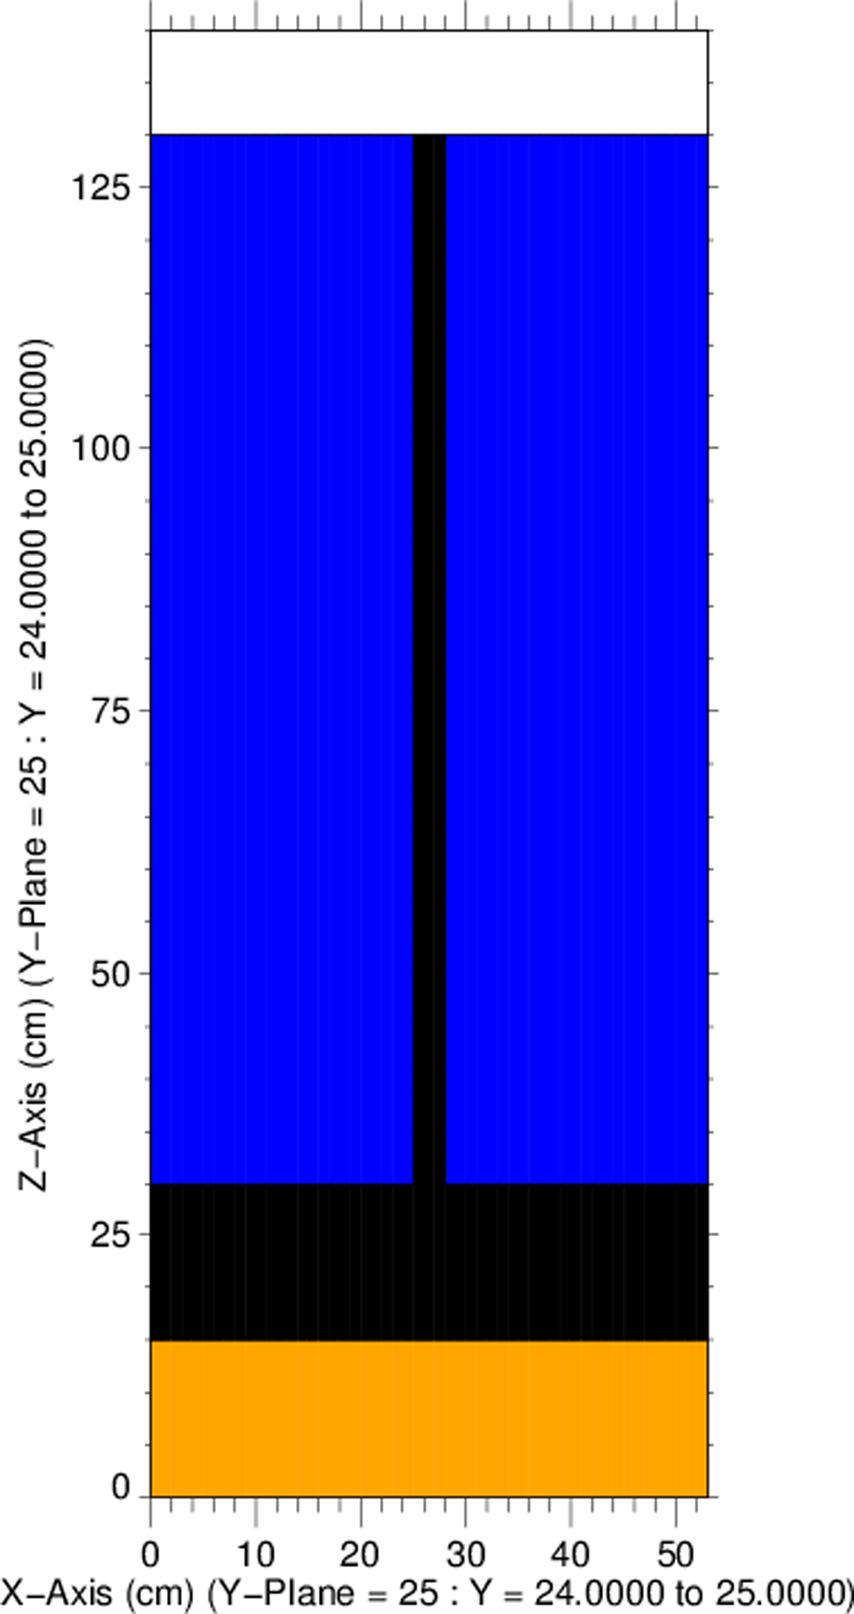
\includegraphics[width=0.4\textwidth]{steel-xz.png}
\caption{Steel plate in water geometry ($x-z$ slice through $y = 25$ cm) 
         \cite{wilsonslaybaugh}.}
\label{steelxz}
\end{figure}

The problem measurements are $53\times50\times140$ cm. The problem is uniform 
in the $y$-direction and materials vary mainly in the $z$-direction. The source
region extends from 0 to 15 cm, the steel shield extends between 15 and 30 cm, 
the water and steel plate extend from 30 to 130 cm, and the air extends from 
130 to 140 cm. The steel plate is 3 cm wide and is centered at $x = 26.5$ cm. 
Vacuum boundary conditions were used at the problem boundaries.

A non-uniform Cartesian mesh was used for the spatial discretization in the 
deterministic calculations. In the $x$-direction, voxel width is 5 cm between
$x = 0$ cm and $x = 25$ cm, 0.5 cm between $x = 25$ cm and $x = 28$ cm, and 5 
cm between $x = 28$ cm and $x = 53$ cm. A uniform spacing of voxel width 1 cm 
was used in the $y$-direction. In the $z$-direction, the spatial cell width is
3 cm between $z = 0$ cm and $z = 30$ cm and 2 cm between $z = 30$ cm and 
$z = 140$ cm.

\begin{table}[!htb]
\centering
\caption{Materials and compositions in the steel plate in water scenario.}
\label{steel-mat}
\begin{tabular}{l|cc}
\textbf{Material} & \multicolumn{2}{c}{\textbf{Isotopes (Atomic Ratio)}} \\ \hline
\multirow{5}{*}{Source}   & U-235   & (0.000247) \\
                          & U-238   & (0.009287) \\
                          & Zr-nat. & (0.004009) \\
                          & H-1     & (0.037394) \\
                          & O-16    & (0.034927) \\ \hline
\multirow{4}{*}{Air}      & N-14    & (0.784431) \\
                          & O-16    & (0.210748) \\
                          & Ar-nat. & (0.004671) \\
                          & C-nat.  & (0.000150) \\ \hline
\multirow{2}{*}{Carbon Steel} & C-nat.  & (0.022831) \\
                              & Fe-nat. & (0.977169) \\ \hline
\multirow{2}{*}{Water}        & H-1     & (2)        \\
                              & O-16    & (1)        \\
\end{tabular}
\end{table}

The material composition of the neutron source block is water, zirconium, and
uranium; calculations used a homogenized combination of the constituent
isotopes. The proportions used in the homogenization are listed in Table
\ref{steel-mat} and are based on the geometry and composition of the Rowlands
UO$_2$ pin cell benchmark specification \cite{pincell}. The source is a U-235
fission spectrum that is uniformly distributed throughout the homogenized
material. The compositions of air, carbon steel, and water were taken from the
Compendium of Material Composition Data for Radiation Transport Modeling
\cite{pnnl}. For this problem, we are interested in the flux solutions at the
end of the steel plate.

%%---------------------------------------------------------------------------%%
\subsection{Dog-Legged Void Neutron (DLVN)}

The next problem modeled is the dog-legged void neutron (DLVN) experimental
benchmark, which was designed to measure neutron streaming in iron with air
voids. The model used in the following calculations was constructed from
publications by Slaybaugh and Wilson \cite{sw-dlvn}, Jarrell et al.\
\cite{j-dlvn}, and Barnett \cite{dlvn1991}. The two materials used in the
problem are elemental iron and polyethylene. The polyethylene composition used
was C$_2$H$_4$. This is listed as ``polyethylene, non-borated'' and is
material 248 in the Compendium of Material Composition Data for Radiation
Transport Modeling \cite{pnnl}.

\begin{figure}[!htb]
\centering
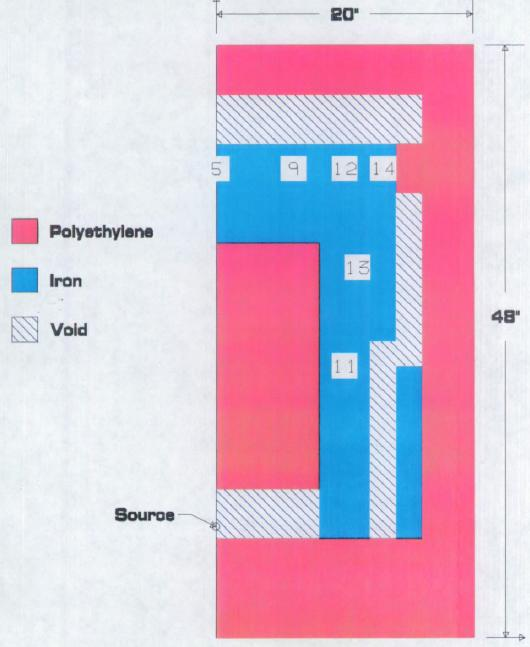
\includegraphics[width=0.5\textwidth]{dlvn.png}
\caption{Centerline cutaway of DLVN setup \cite{sw-dlvn}.}
\label{dlvn}
\end{figure}

The problem measurements are $40\times54\times48$ inches. A uniform spatial
mesh was imposed over the entire problem, with voxels measuring 1 inch per
side. The neutron source in this problem is a Cf-252 point source located at
the center of the $x-$ and $y-$directions and at $z = 9$ inches. This point
source was approximated as a small volumetric source in the tests in this
work. We are interested in the forward flux solutions at the various detector
locations shown in Figure \ref{dlvn}; this test case is of interest
because the streaming pathways in the configuration make the problem
computationally challenging. It is particularly interesting because the DLVN
configuration contains both physical streaming in air and energy streaming in
iron. 

The DLVN configuration is symmetric about the $y-z$ plane at $x = 0$
and so is usually simulated with a reflecting boundary at $x = 0$ and vacuum
boundaries on all other sides of the configuration. For the tests in this work,
the use of reflecting boundary conditions was not available, so the model used 
was constructed to represent the entire geometry.
Vacuum boundary conditions were applied to the outside of the entire problem.

%%---------------------------------------------------------------------------%%
\subsection{Simplified Portal Monitor}

The final problem described here, a simplified portal monitor scenario, is a
\textit{photon-only} transport problem (the first two test problems are
neutron-only transport problems). Portal monitors are large detector
panels used to screen cargo for illicit radioactive materials. The problem
models a cargo container holding a Ba-133 photon point source and large blocks
of homogenized iron and polyethylene. The geometry and material configuration
used in this test is the same as the example problem listed in Section 7.2 of
the ADVANTG technical report \cite{advantg}. Diagrams of the simplified portal
monitor problem are shown in Figure \ref{p1}. The problem is of interest
because of the computational challenge generated by the particle streaming
pathways in the problem's geometry as well as the importance of portal
monitors.

\begin{figure}[!htb]
\centering
\begin{subfigure}{0.475\textwidth}
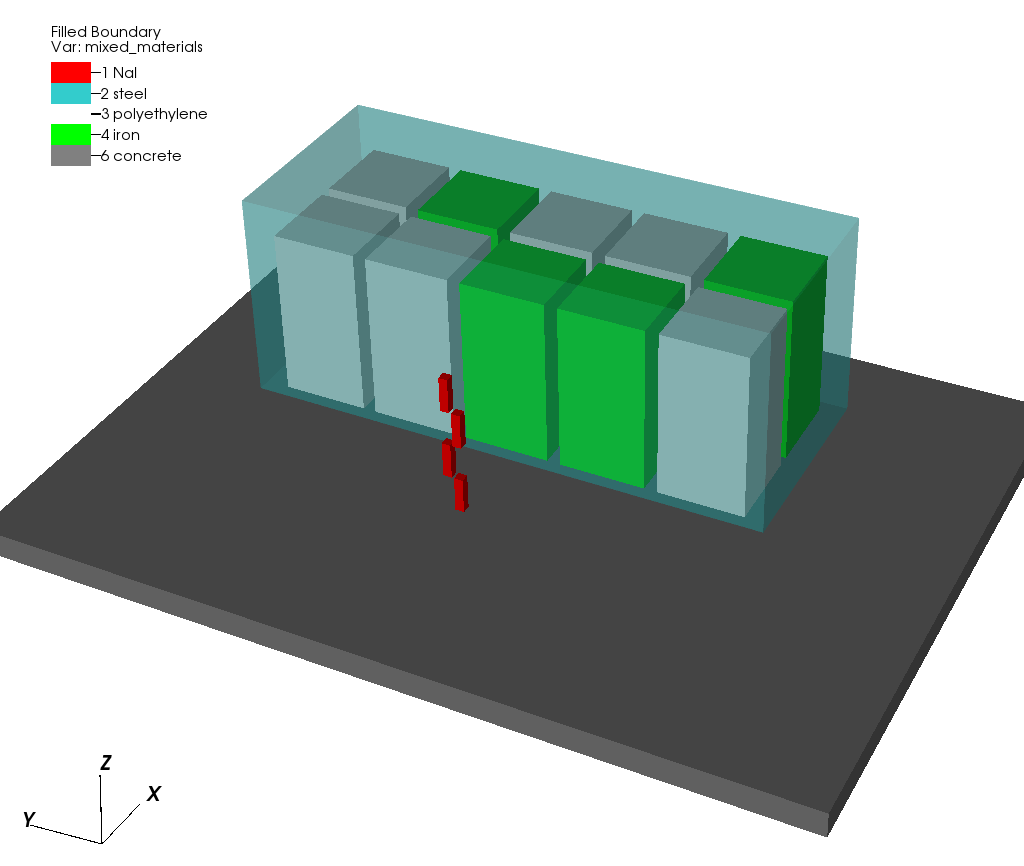
\includegraphics[width=\textwidth]{portal1.png}
\end{subfigure}
\begin{subfigure}{0.475\textwidth}
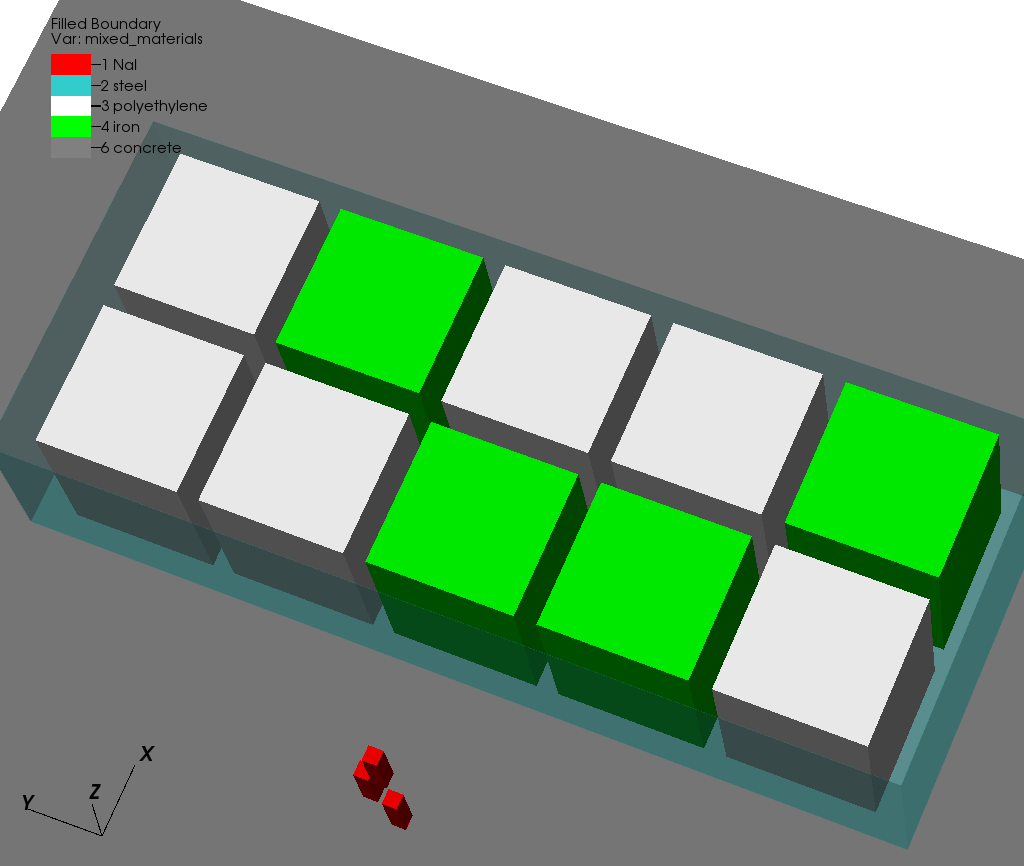
\includegraphics[width=\textwidth]{portal2.png}
\end{subfigure}
\caption{Top and side views of simplified portal problem \cite{advantg}.}
\label{p1}
\end{figure}

In Figure \ref{p1}, the different colors represent different materials. The NaI
detectors are red and the gray material is concrete. The two types of material
blocks are iron, shown in green, and polyethylene, shown in white. The steel
cargo container surrounds the particle source and material blocks and is a
semitransparent blue.

A non-uniform Cartesian mesh that captures all of the problem's material
boundaries was constructed for this simulation. The voxels are nominally 10 cm
thick within the cargo container. Additional mesh planes parallel to the
$x-$axis were added to the gaps between the homogenized iron and polyethylene
blocks \cite{advantg}. Vacuum boundary conditions are present at all problem
edges.

\subsection{Calculation Parameters}
\label{params}

To ensure consistent comparisons between MC VR parameters generated from the
different quadrature types and sets, the deterministic calculations used the
same spatial computational block structure and energy discretization.
All of the deterministic calculations used 32 processes on a 2.8GHz AMD
Opteron\texttrademark\ 6320 Processor \cite{amd}, two for each logical CPU
unit. Denovo uses the Koch-Baker-Alcouffe (KBA) parallel sweep algorithm for
high parallel efficiency in calculating transport sweeps \cite{denovo}. All
deterministic calculations were set to use the same Denovo computational block
structure of 8 blocks in the $x-$dimension, 4 blocks in the $y-$dimension, and
1 block in the $z-$dimension such that the total number of computational blocks
equals the number of processes.

Because energy discretization is treated the same way between the traditional
discrete ordinates formulation and the LDO equations, it was assumed that
energy group structure would not greatly affect the comparative results. All
but one of the test cases use the same coarse energy group structure specified
in the ``27n19g'' library; the groups in this library are listed in Table A-1
of Appendix A of the ADVANTG technical report \cite{advantg}. The exception to
this is the simplified portal problem. The highest energy emission line of
Ba-133 is 383.8 keV, so weight window bounds above this energy would not be
used in the Monte Carlo simulation. Thus, the highest energy group of the
deterministic calculations was set to group number 41, which has an upper
energy of 400 keV \cite{advantg}.

In the deterministic calculations, forward solutions for the test cases were
generated using quadruple range (QR), Galerkin, linear-discontinuous finite 
element (LDFE), and LDO quadrature sets. All test cases were run with the same 
quadrature sets; increasing sizes of quadrature sets were used to ascertain the
angular mesh refinement necessary for a given quadrature type to converge to a 
solution. The orders and sizes of the LDO quadrature sets used are listed in
Table \ref{ldo-n}.

\begin{table}[!htb]
\centering
\caption{Properties of LDO quadrature sets used in deterministic calculations.}
\begin{tabular}{cc}
\multicolumn{1}{l}{\textbf{Quadrature Order ($\mathbf{N}$)}} & 
\multicolumn{1}{l}{\textbf{Number of Points}} \\
\hline
3 & 16 \\
5 & 36 \\
8 & 81 \\
9 & 100 \\
11 & 144 \\
12 & 169 \\
13 & 196 \\
14 & 225 \\
\end{tabular}
\label{ldo-n}
\end{table}

QR quadrature sets were chosen to generate reference results against which
the LDO results are compared. QR was selected because it is commonly used 
in hybrid methods for Monte Carlo variance reduction parameter generation and 
therefore provides a relevant baseline. The Exnihilo framework allows the user
to select the number of polar and azimuthal angles in each octant when using a
QR quadrature set; for these studies, the number of polar and azimuthal angles
per octant were each set to the same value, with the values ranging from one
per octant (for a total of eight angles) to nine per octant (for a total of
648 angles). 

LDFE and Galerkin quadrature sets were also chosen because of their interesting
mathematical properties. Compared to QR quadrature sets, LDFE quadrature sets
have been shown to exhibit more accurate solutions for the scalar flux in both 
simple and more complex geometry and material configurations \cite{ldfe}; they 
approximate the angular flux using direction cosines and are determined by
requiring that the integration of the related interpolation basis functions is
equal to the surface area of a unit sphere. For LDFE quadrature sets, if $N$ is
the order of the quadrature, there are $4^{(N+1)}$ angles per octant
\cite{exum}. In this work, the LDFE quadrature orders used were one (128 total
angles) and two (8192 total angles).

Galerkin quadrature sets offer several advantages relative to the standard
\sn\ method for problems with highly anisotropic scattering \cite{morel}.
Similar to the LDO equations, the 
``hybrid collocation-Galerkin-S$_\mathrm{N}$'' method developed by Morel 
has the same algebraic structure as the traditional discrete ordinates
equations but employs a nonstandard scattering treatment. For an \sn\ order
$N$, a given Galerkin quadrature set has a total of $N(N+2)$ angles. The
Galerkin quadrature orders used were 2 and 4; the
Galerkin quadrature sets used in this work have 8 and 24 total angles,
respectively.

The step characteristics (SC) spatial discretization was used in all of the
deterministic calculations based on the recommendation listed in Section 9.1.3
of the Exnihilo user manual \cite{exum}. In the DLVN and portal monitor
problems, the point sources are approximated as small spherical volumetric
sources. Except for the Galerkin quadratures, all calculations used a P$_5$
scattering expansion. At the time of this writing, Galerkin quadrature sets
are implemented in the Exnihilo framework with the restriction that the \pn\
order be one greater than the \sn\ order. That is, for the Galerkin quadrature
set of \sn\ order 2, the corresponding \pn\ order is set equal to 3, and for
the Galerkin quadrature set of \sn\ order 4, the \pn\ order is 5. It is not
anticipated that this will greatly impact the results; the Galerkin
quadrature sets used here feature relatively coarse angular meshes and are
included to provide a comparison with another quadrature type that uses a
nonstandard scattering treatment.

The Monte Carlo calculations in this work were run on one Dell PowerEdge C6220
server blade node with two Intel Xeon 10-core Ivy Bridge processors (a total
of 20 cores) \cite{savio}. All calculations were specified to use 21 MPI
tasks; MCNP reserves one ``master'' process for communication and transports
particles with the remaining available tasks \cite{mcnp}. For the purpose of
parallel efficiency, one transport process per hardware core was used here.

All of the Monte Carlo calculations were run with a fixed number of particle
histories. For the steel plate in water and simplified portal
monitor cases, all calculations used 1\E{9} particle histories. The DLVN
experimental benchmark case was simulated with 1\E{10} neutron histories as it
was modeled after calculations performed by Slaybaugh and Wilson
\cite{sw-dlvn}. All Monte Carlo tally results, $\xbar$, are reported with the
one standard deviation confidence interval, $\xbar(1\pm R)$, where the relative
error, $R$, is defined as $S_{\xbar}/\xbar$ and $S_{\xbar}$ is the standard
deviation of the tally result estimate \cite{mcnp}.

In the \fwc\ calculations for the DLVN and simplified portal monitor
scenarios, we examine Monte Carlo results corresponding to variance reduction
parameters from a chosen representative subset of the quadrature sets. For
these comparisons, quadrature sets of similar angular mesh refinement were
chosen such that the quadrature sets have approximately the same total number
of angles, with the exception of the Galerkin quadrature set. The QR
quadrature set is of order 4 and has 128 angles, the LDFE set is order 1 with
128 angles, and the LDO set is of order 11 with 144 angles. The Galerkin
quadrature set chosen as the representative example here is of order 4 and has
24 angles. This set was chosen because its corresponding \pn\ order is 5 and
so the scattering data used matches that of the other quadrature types.

%%---------------------------------------------------------------------------%%
\section{Results}
\label{sec:results}

For the three test cases described above, we will examine the flux
tally results and Figure of Merit (FOM) values reported by MCNP. We note that
Figures of Merit are calculated as
%
\begin{equation}
\text{FOM} = \frac{1}{R^2T},
\label{eq:fom}
\end{equation}
%
where $R$ is the estimated relative error and $T$ is the computer time taken
to complete the calculation \cite{mcnp}. Flux tally and FOM values are
presented for the test cases in the contexts of both the CADIS and
\fwc\ methods, with additional focus on how the results vary as a function of
angular mesh refinement used in the deterministic calculations from which
Monte Carlo variance reduction parameters were generated. For additional
results and analysis, including comparisons with experimentally-gathered
data where available, we refer the reader to Rowland's previous related
publication \cite{kr}.

When considering the results presented, keep in mind that some of these
problems are nearly pathological in difficulty, especially the steel plate
embedded in water. In some cases, no quadrature is able to create VR
parameters to obtain a valid solution in a reasonable time. In these
circumstances, we still compare performance in terms of FOM. This
is because, with enough simulated particles, a correct solution would be obtained.
Therefore, a better FOM still indicates which method to choose to get
the correct answer more quickly. The results below elucidate when the LDO
equations are a good choice, and we acknowledge that we have not yet found a
method that always works when problems have strong angular anisotropy. The
contribution here is that using the LDO equations to generate Monte Carlo VR
parameters increases the number of problems we can solve with CADIS and \fwc.

%%---------------------------------------------------------------------------%%
\subsection{Steel Plate Embedded in Water}

%%---------------------------------------------------------------------------%%
\subsubsection{CADIS}

For the CADIS calculations for the steel plate embedded in water, the adjoint
source was set to be the detector tally. Figure \ref{steel-cadis} shows
the MCNP-reported flux tally for the detector at the end of the steel plate
for each angular mesh refinement for each quadrature type. We note that the
Monte Carlo calculations with VR parameters from the Galerkin quadrature
set of order 2 and the LDO quadrature set of order 5 were not able to finish
in a timely manner for the hardware configuration used in this work, so Monte
Carlo results for those two data points are not included here. The flux tally
results are plotted as a function of angular mesh refinement to investigate
the effect of angular mesh refinement on flux tally solution for the different
quadrature types; we observe that the angular mesh refinement does not greatly
affect the calculated flux tally value or the associated error. 

Additionally, it is instructive to look at the Figures of Merit for the
various results to observe trends that could translate to other problems where
correct results are obtained. Figure \ref{steel-cadis} shows the reported
FOM value for the detector tally for the various quadrature sets and orders.
The VR parameters corresponding to the LDFE quadrature set of order 1 (128
quadrature points) result in the highest FOM value while those of the QR set of
order 1 (8 quadrature points) result in the lowest FOM value.

\begin{figure}[!htb]
\centering
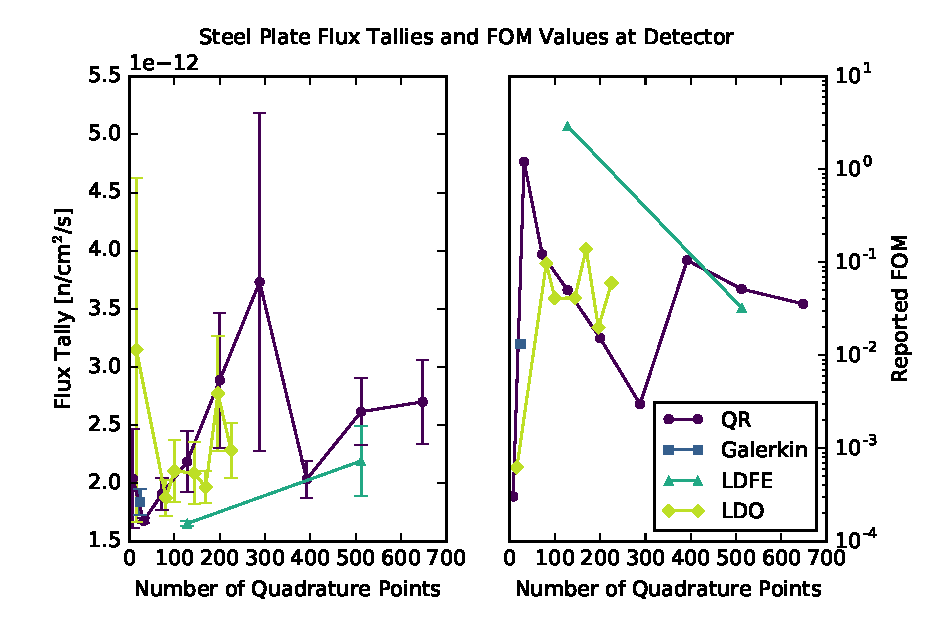
\includegraphics[max height=0.445\textheight]{steel-cadis.eps}
\caption{MCNP-reported forward flux tally and FOM values at the end of the
         steel plate.}
\label{steel-cadis}
\end{figure}

To conclude this subsection, we consider the overall trends in angular mesh
refinement in Figure \ref{steel-cadis}. It appears that the angular mesh
refinement does not have a large influence on the flux tally value in this
problem, as all of the tally results using VR parameters fall within the same
order of magnitude and do not exhibit any trends as a function of the number
of discrete angles used. This indicates that any improvement gained by more
accurate angular information is offset by the increased computational cost.
The Figures of Merit vary somewhat more greatly. Specifically, the LDO VR
parameters appear to gather around FOM values of 0.005 even as the number of
discrete angles used is increased. Thus, for the steel plate in water problem
solved with the CADIS method, one could use a relatively low-order
(\textit{i.e.}, order 8, which is 81 quadrature points) LDO quadrature set to
generate Monte Carlo VR parameters that result in a Figure of Merit comparable
to or better than those produced by finer angular meshes.

\FloatBarrier
%%---------------------------------------------------------------------------%%
\subsubsection{\fwc}

For the \fwc\ calculations for the steel plate in water, the adjoint source
was set to be a mesh tally over all of the air beyond the steel plate. The
discretization for the adjoint source mesh tally is the same as that listed in
Section \ref{sec:steel_params}. Specifically, the adjoint source mesh is
identical to the overall problem mesh in the $x-$ and $y-$directions but
starts at $z = 130$ cm and extends to the problem boundary at $z = 140$ cm.
The Monte Carlo calculation with VR parameters from the Galerkin
quadrature set of order 2 was not able to finish in a timely manner for the
hardware configuration used in this work, so Monte Carlo results for this data
point are not included here.

Figure \ref{steel-fwc} shows the total tally summed over all air in the
problem for the Monte Carlo calculations with VR parameters. The calculations
with VR parameters are plotted as a function of angular mesh refinement. Like
in the CADIS method, the angular mesh refinement has little impact on the
tally results. If using an LDO quadrature set to generate VR parameters with
the \fwc\ method in a similar case, a low-order LDO angular mesh could be
used to good effect.

To analyze the performance of the representative quadrature sets' variance
reduction parameters for the steel plate in water case using the \fwc\ method,
we will look at the average FOM values over the entire adjoint source mesh
tally. The Figures of Merit were calculated by taking the average relative
error over all spatial cells in the air block mesh tally and using that mean
value in combination with the MCNP-reported computer time. Figure 
\ref{steel-fwc} shows these average Figures of Merit as a function of the
number of angles used in generating the VR parameters.

\begin{figure}[!htb]
\centering
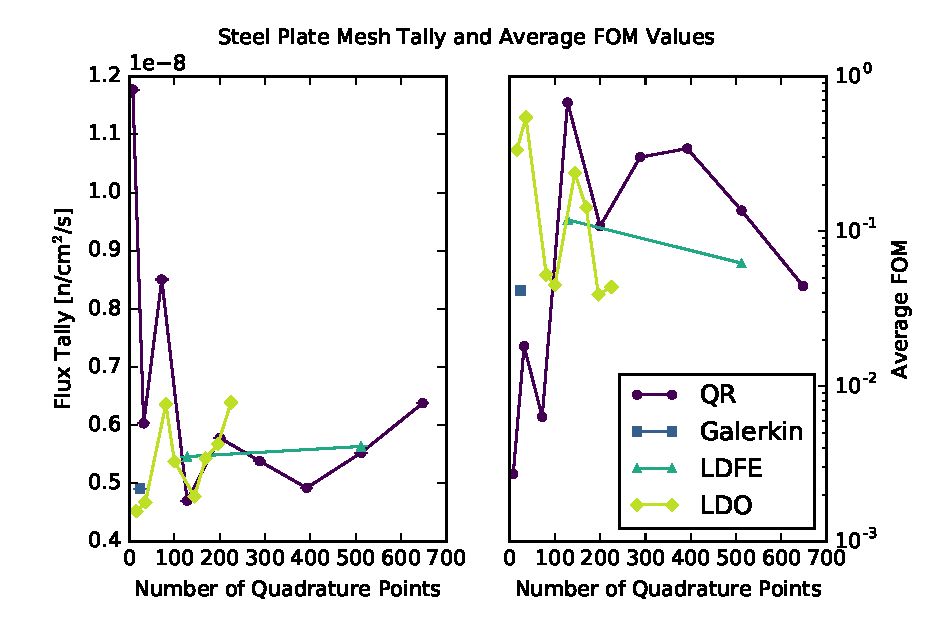
\includegraphics[max height=0.445\textheight]{steel-fwcadis.eps}
\caption{Scalar flux and average FOM values for the mesh tally in the \fwc\
         steel plate test.}
\label{steel-fwc}
\end{figure}

We see a different trend here than with CADIS in that the highest average FOM
values tend to come from quadrature sets with mid-range angular mesh
refinement; the coarsest and finest angular meshes produce Monte Carlo VR
parameters that result in reduced Figures of Merit. This indicates that too
low an angular resolution likely does not provide enough accuracy, while a
high resolution adds computational cost without much accuracy benefit.
Considering Figure \ref{steel-fwc}, we note that one would wish to use a
lower-order (\textit{e.g.}, order 5, which is 36 quadrature points) LDO
quadrature set to generate variance reduction parameters for a Monte Carlo
mesh tally using the \fwc\ method.

This is a true challenge problem. We note that for bot  h the CADIS and \fwc\ results, the solution was not clearly obtained. This problem is very difficult to solve---Wilson and Slaybaugh \cite{wilsonslaybaugh} were unable to obtain accurate solutions using a reasonable number of particles with analog Monte Carlo or CADIS or \fwc\ despite many deterministic parameter choices. The meaning of the recommendations here is that, with enough particles, a correct solution would eventually be obtained and using the method with the best FOM will get there the fastest. 

\FloatBarrier
%%---------------------------------------------------------------------------%%
\subsection{Dog-Legged Void Neutron (DLVN)}

%%---------------------------------------------------------------------------%%
\subsubsection{CADIS}

To study the DLVN problem in the context of the CADIS method, the adjoint
source was set to be the tally located at detector \#14 in the original
experiment. Detector \#14 was chosen because it is centrally located among the
detectors and farthest from the forward source. Figure \ref{dlvn-cadis}
shows the MCNP-reported tally for the forward scalar flux at the location of
detector \#14.

\begin{figure}[!htb]
\centering
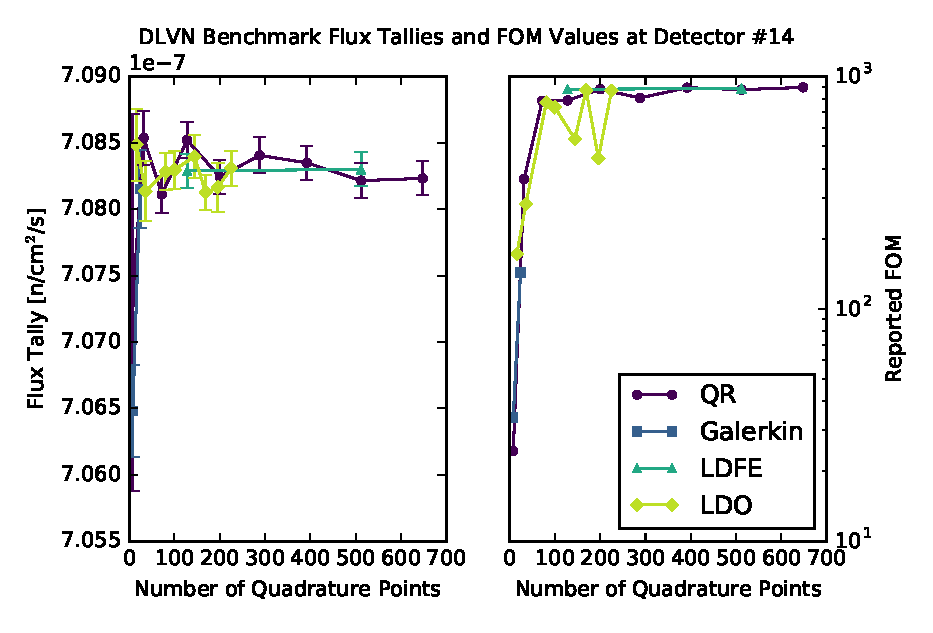
\includegraphics[max height=0.445\textheight]{dlvn-cadis.eps}
\caption{Flux tally and FOM values for the DLVN problem detector \#14 tally
         with the CADIS method.}
\label{dlvn-cadis}
\end{figure}

Figure \ref{dlvn-cadis} shows similar convergence
behavior with respect to angular mesh refinement for the tally calculations
and Figure of Merit values resulting from calculations using VR parameters.
Beyond the lowest-order angular mesh refinement for each quadrature type
studied here, the tally result for this detector location using the CADIS
method is not affected by further refining the angular mesh. The Figures of
Merit for the tally calculations reach a similar upper bound, but this happens
more slowly with respect to angular mesh refinement for the LDO quadrature
sets. Like the tally in the steel plate case above, the LDO quadrature set of
order 8 (81 quadrature points) is the best choice with respect to flux tally
result and FOM value for detector \#14 in the DLVN experimental benchmark
problem in the CADIS context.

\FloatBarrier
%%---------------------------------------------------------------------------%%
\subsubsection{\fwc}

Considering the DLVN case with the \fwc\ method, the adjoint source was
specified to be the combination of all of the detector locations in the
problem. Figures \ref{dlvn-fwc-5} and \ref{dlvn-fwc-9} exhibit the same lack of trend in
flux tally as a function of angular mesh refinement. That is, in general, for
detector locations \#5 and \#9, using more discrete angles in the \fwc\
deterministic calculations does not greatly impact the flux tally result from
MCNP. Figures \ref{dlvn-fwc-13} and \ref{dlvn-fwc-14} show similar behavior
with the exception of the coarsest angular meshes. For these detector
locations, any angular mesh refinement other than the coarsest angular mesh
will produce a consistent forward scalar flux tally result. Figures
\ref{dlvn-fwc-11} and \ref{dlvn-fwc-12} show slightly more variation in flux
tally result with angular mesh refinement. These two detector locations'
tallies also have higher statistical error relative to those at the other
detector locations. Overall, though, the flux tallies at detectors \#11 and
\#12 are not heavily impacted by the refinement of the angular mesh used in
generating the Monte Carlo VR parameters, but a mid-range number of
quadrature points should be used to avoid the large statistical errors seen at
the extreme ends of the angular mesh refinement spectrum.

Like their corresponding flux tally graphs, Figures \ref{dlvn-fwc-5},
\ref{dlvn-fwc-9}, and \ref{dlvn-fwc-13} show almost no variation in FOM with
angular mesh refinement for the tallies at detector locations \#5, \#9, and
\#13. This is not surprising in the \fwc\ context, as the global VR parameters
produce more uniform statistical errors and
stable flux tally results at these locations. Figure \ref{dlvn-fwc-11} shows
variation in FOM with angular mesh refinement that is more varied, which
corresponds to the larger statistical uncertainties in the flux tally values
for detector \#11. This is likely due to the close proximity of detector \#11
to the bend in the ``dog-legged'' void; problems with small air gaps between
shielding materials, such as the DLVN experimental benchmark, are historically
difficult to solve well with hybrid methods.
Figure \ref{dlvn-fwc-12} shows little variation in FOM with
angular mesh refinement with the exception of the finest QR set. Lastly,
\ref{dlvn-fwc-14} shows an upper FOM limit of approximately 200 across all
quadrature types, with the Figure of Merit largely consistent across
quadrature types with the exception of QR angular meshes.

To examine the FOM values in a more quantifiable way, Table 
\ref{dlvn-fwc-fom-table} lists the FOM values for all detector locations for
each of the representative quadrature sets listed in Section \ref{params}.
The maximum FOM value in each detector location column is emphasized. Of the
six detector locations, the representative LDO quadrature set achieves the
highest FOM for two of the locations. The representative QR quadrature set is
the only other type to also deliver the highest Figure of Merit for two out of
six detectors; the Galerkin and LDFE quadrature set VR parameters each
only achieve the highest FOM for one detector location. So, the representative
LDO quadrature set's VR parameters perform comparably to those from the
representative QR quadrature set with respect to obtaining high FOM values for
multiple detector locations using the \fwc\ method for the DLVN problem.

\begin{table}[!hbt]
\centering
\captionsetup{justification=centering}
\caption{\fwc\ FOM values for representative quadratures for the DLVN problem,
         with best performance at each detector indicated with bold font.}
\label{dlvn-fwc-fom-table}
\begin{tabular}{l|cccccc}
\multicolumn{1}{l|}{Quadrature}
& \multicolumn{1}{l}{Detector 5}
& \multicolumn{1}{l}{Detector 9}
& \multicolumn{1}{l}{Detector 11}
& \multicolumn{1}{l}{Detector 12}
& \multicolumn{1}{l}{Detector 13}
& \multicolumn{1}{l}{Detector 14}
\\ \hline
\begin{tabular}[c]{@{}l@{}}   QR \end{tabular} 
& \begin{tabular}[c]{@{}c@{}} 483.012 \end{tabular} % fom for #5
& \begin{tabular}[c]{@{}c@{}} 709.51 \end{tabular} % fom for #9
& \begin{tabular}[c]{@{}c@{}} \textbf{202.66} \end{tabular} % fom for #11
& \begin{tabular}[c]{@{}c@{}} 747.914 \end{tabular} % fom for #12
& \begin{tabular}[c]{@{}c@{}} 380.843 \end{tabular} % fom for #13
& \begin{tabular}[c]{@{}c@{}} \textbf{185.40} \end{tabular} % fom for #14
\\
\begin{tabular}[c]{@{}l@{}}   Galerkin \end{tabular} 
& \begin{tabular}[c]{@{}c@{}} \textbf{527.794} \end{tabular} % fom for #5
& \begin{tabular}[c]{@{}c@{}} 649.88 \end{tabular} % fom for #9
& \begin{tabular}[c]{@{}c@{}} 5.9934 \end{tabular} % fom for #11
& \begin{tabular}[c]{@{}c@{}} 798.878 \end{tabular} % fom for #12
& \begin{tabular}[c]{@{}c@{}} 326.107 \end{tabular} % fom for #13
& \begin{tabular}[c]{@{}c@{}} 52.098 \end{tabular} % fom for #14
\\
\begin{tabular}[c]{@{}l@{}}   LDFE \end{tabular} 
& \begin{tabular}[c]{@{}c@{}} 310.276 \end{tabular} % fom for #5
& \begin{tabular}[c]{@{}c@{}} 710.43 \end{tabular} % fom for #9
& \begin{tabular}[c]{@{}c@{}} 6.6749 \end{tabular} % fom for #11
& \begin{tabular}[c]{@{}c@{}} 926.278 \end{tabular} % fom for #12
& \begin{tabular}[c]{@{}c@{}} \textbf{391.624} \end{tabular} % fom for #13
& \begin{tabular}[c]{@{}c@{}} 166.51 \end{tabular} % fom for #14
\\
\begin{tabular}[c]{@{}l@{}}   LDO \end{tabular}
& \begin{tabular}[c]{@{}c@{}} 478.242 \end{tabular} % fom for #5
& \begin{tabular}[c]{@{}c@{}} \textbf{721.22} \end{tabular} % fom for #9
& \begin{tabular}[c]{@{}c@{}} 19.959 \end{tabular} % fom for #11
& \begin{tabular}[c]{@{}c@{}} \textbf{943.959} \end{tabular} % fom for #12
& \begin{tabular}[c]{@{}c@{}} 369.423 \end{tabular} % fom for #13
& \begin{tabular}[c]{@{}c@{}} 110.40 \end{tabular} % fom for #14
\end{tabular}
\end{table}

In summary, for test cases such as the DLVN problem in which the
\fwc\ method is used to generate Monte Carlo variance reduction parameters to
optimize the response at multiple flux tally detector locations, a relatively
coarse quadrature set of any of the types studied here can be used to
sufficient effect. However, the coarsest available quadrature sets should be
avoided; flux tally results and Figures of Merit for the various detector
locations tend to level out as a function of angular mesh refinement beyond
the quadrature sets with the fewest number of angles. In particular, if using
an LDO quadrature set in another similar problem, we would suggest using a
point set of order 5 (36 quadrature points) or order 8 (81 quadrature points).

\begin{figure}[!htb]
\begin{subfigure}{\linewidth}
\centering
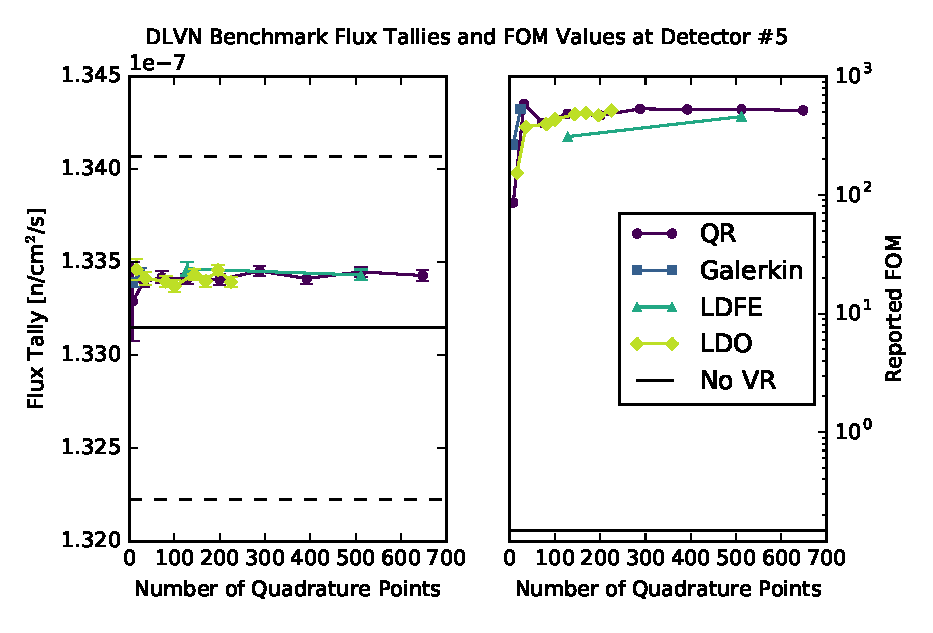
\includegraphics[max height=0.445\textheight]
{dlvn-fwcadis-5.eps}
\subcaption{MCNP-reported forward flux tally and FOM values at detector \#5.}
\label{dlvn-fwc-5}
\end{subfigure} 
\\
\begin{subfigure}{\linewidth}
\centering
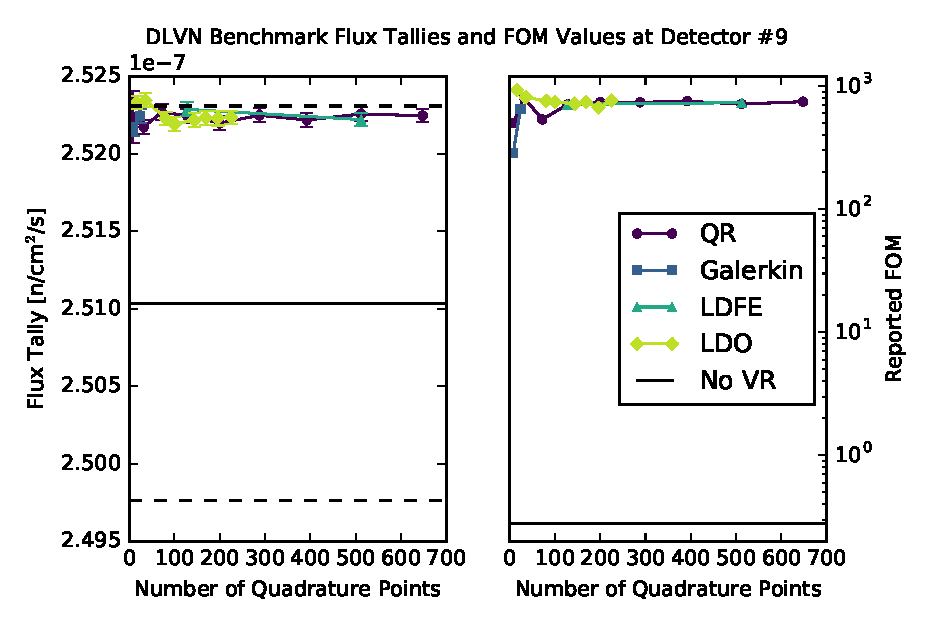
\includegraphics[max height=0.445\textheight]
{dlvn-fwcadis-9.eps}
\subcaption{MCNP-reported forward flux tally and FOM values at detector \#9.}
\label{dlvn-fwc-9}
\end{subfigure}
\end{figure}
\clearpage
\begin{figure}[!htb]
\ContinuedFloat
\begin{subfigure}{\linewidth}
\centering
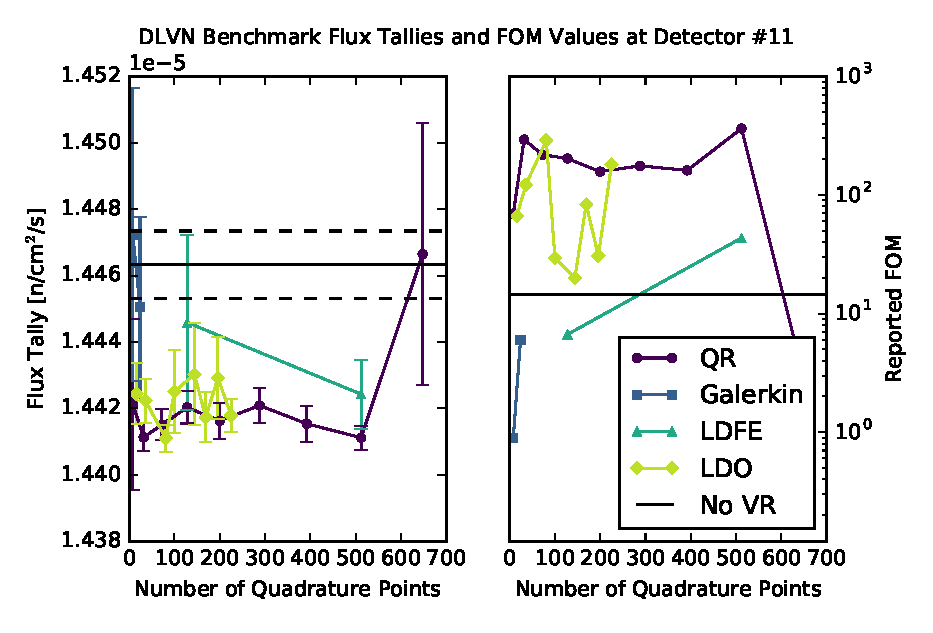
\includegraphics[max height=0.445\textheight]
{dlvn-fwcadis-11.eps}
\subcaption{MCNP-reported forward flux tally and FOM values at detector \#11.}
\label{dlvn-fwc-11}
\end{subfigure}
\\
\begin{subfigure}{\linewidth}
\centering
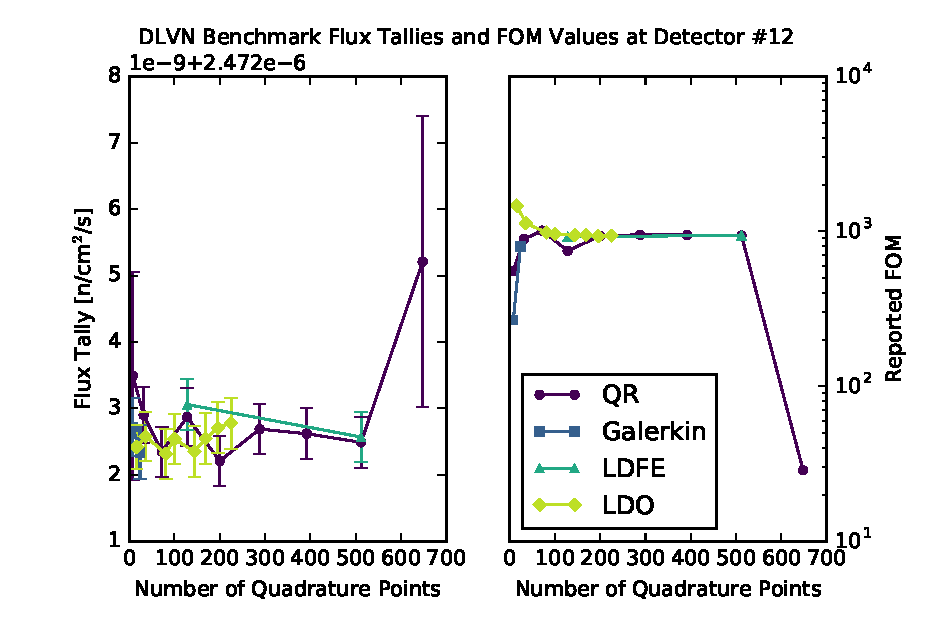
\includegraphics[max height=0.445\textheight]
{dlvn-fwcadis-12.eps}
\subcaption{MCNP-reported forward flux tally and FOM values at detector \#12.}
\label{dlvn-fwc-12}
\end{subfigure}
\end{figure}
\clearpage
\begin{figure}[!htb]
\ContinuedFloat
\begin{subfigure}{\linewidth}
\centering
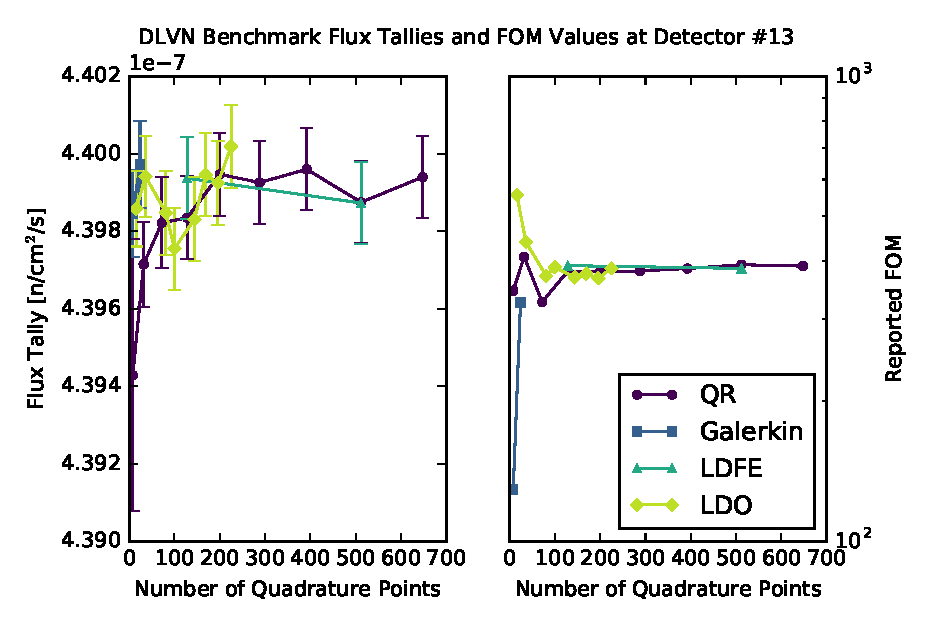
\includegraphics[max height=0.445\textheight]
{dlvn-fwcadis-13.eps}
\subcaption{MCNP-reported forward flux tally and FOM values at detector \#13.}
\label{dlvn-fwc-13}
\end{subfigure} 
\\
\begin{subfigure}{\linewidth}
\centering
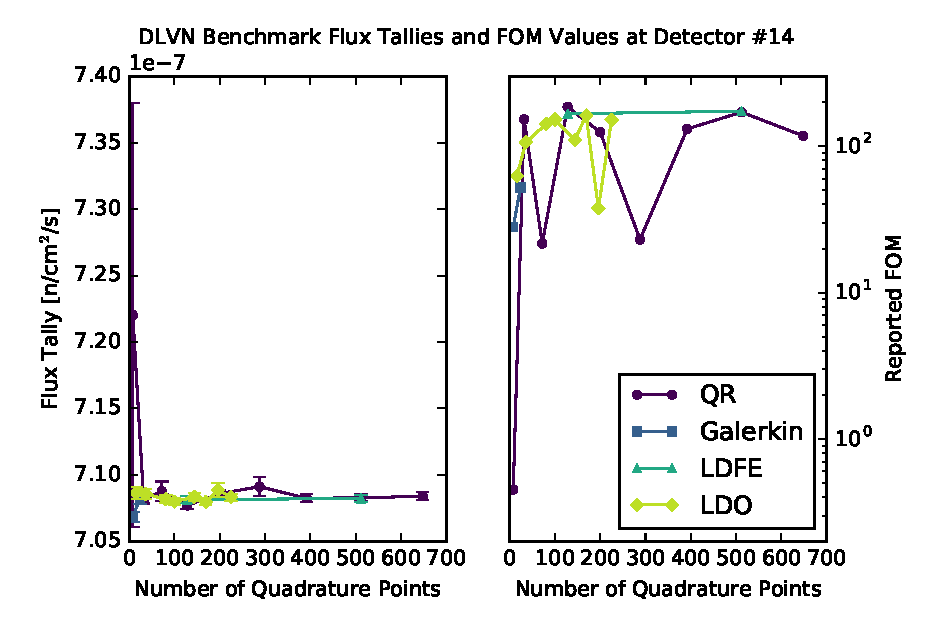
\includegraphics[max height=0.445\textheight]
{dlvn-fwcadis-14.eps}
\subcaption{MCNP-reported forward flux tally and FOM values at detector \#14.}
\label{dlvn-fwc-14}
\end{subfigure}
\caption{\fwc\ flux tallies and FOM values for the DLVN problem.}
\label{dlvn-fwc-tally}
\end{figure}

\FloatBarrier
%%---------------------------------------------------------------------------%%
\subsection{Simplified Portal Monitor}

%%---------------------------------------------------------------------------%%
\subsubsection{CADIS}

To study calculations for the simplified portal monitor test case in the
context of the CADIS method, the adjoint source was set to be the top detector
in the small array. Figure \ref{cargo-cadis} shows the MCNP-reported forward scalar flux tally
values and Figures of Merit. As with the other test cases, the values are
plotted as a function of the number of quadrature points used to generate the
VR parameters in order to explore the effect of angular mesh refinement on
flux tally and FOM.

\begin{figure}[!htb]
\centering
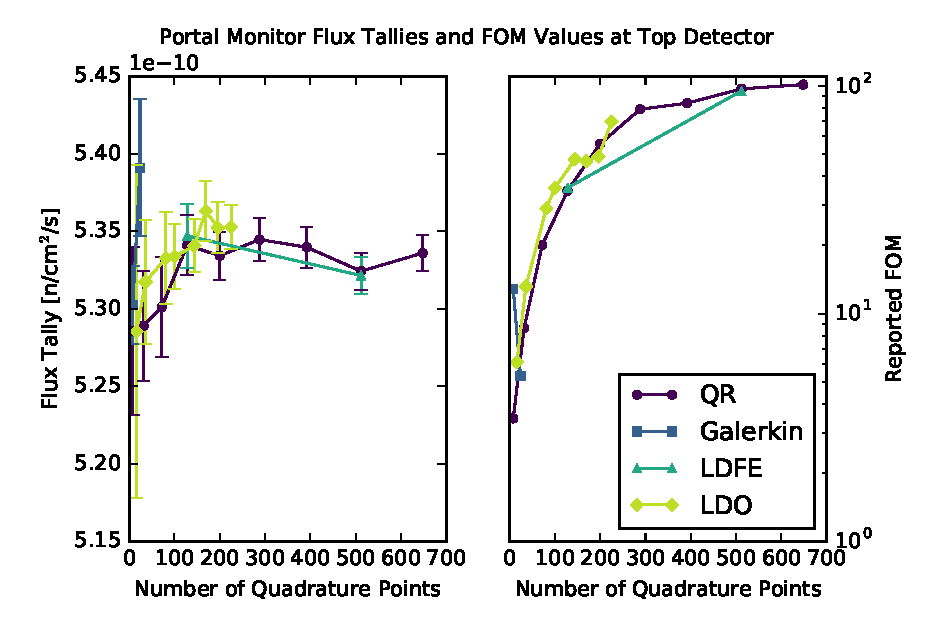
\includegraphics[max height=0.445\textheight]{portal-cadis.eps}
\caption{Flux tally and FOM values in the portal monitor top detector using
         the CADIS method.}
\label{cargo-cadis}
\end{figure}

Similar to other test cases, the flux tally values reported in Figure 
\ref{cargo-cadis} show a trend of converging to a stable value after the
first few coarsest angular meshes. The flux tally values from the
calculations using VR appear to require a minimum value of approximately 100
discrete angular values in order to stabilize. Figure \ref{cargo-cadis}
shows a strong correlation between the number of quadrature points and the
flux tally FOM, eventually approaching an upper limit around 100. The LDO
Figures of Merit increase most rapidly with the number of quadrature points
used, so one would want to use a higher-order LDO quadrature set to generate
Monte Carlo VR parameters.

\FloatBarrier
%%---------------------------------------------------------------------------%%
\subsubsection{\fwc}

To generate Monte Carlo variance reduction parameters for the simplified portal
monitor using the \fwc\ method, the adjoint source was set to be all four
detector locations in the problem's detector array. Figure \ref{cargo-fwc} shows MCNP-reported forward scalar flux tallies and
Figures of Merit for all four detectors in the array. The flux tallies and FOM
values are each plotted as a function of the number of discrete angles used in
the quadrature sets that were used to generate VR parameters. At all
detector locations, the forward flux tallies and FOM values show the same
trend of leveling off to a stable value once the angular mesh used for the
\fwc\ VR parameters has been refined past the few coarsest numbers of discrete
angles.

Table \ref{cargo-fwc-fom-table} lists the Figures of Merit for the various
detector locations for the representative quadrature sets. We see that the
VR parameters from the representative LDO quadrature set produce the
highest Figures of Merit for three out of four detector locations, with the
representative QR quadrature set's VR parameters achieving the highest FOM
for the bottom detector in the array.

\begin{table}[!hbt]
\centering
\captionsetup{justification=centering}
\caption{\fwc\ FOM values for representative quadratures for the portal
         monitor, with best performance at each detector indicated with bold
         font.}
\label{cargo-fwc-fom-table}
\begin{tabular}{l|cccc}
\multicolumn{1}{l|}{Quadrature}
& \multicolumn{1}{l}{Top Detector}
& \multicolumn{1}{l}{\nth{2} Detector}
& \multicolumn{1}{l}{\nth{3} Detector}
& \multicolumn{1}{l}{Bottom Detector}
\\ \hline
\begin{tabular}[c]{@{}l@{}}   QR \end{tabular} 
& \begin{tabular}[c]{@{}c@{}} 76.1145 \end{tabular} % fom for #14
& \begin{tabular}[c]{@{}c@{}} 121.241 \end{tabular} % fom for #24
& \begin{tabular}[c]{@{}c@{}} 128.9 \end{tabular} % fom for #34
& \begin{tabular}[c]{@{}c@{}} \textbf{81.125} \end{tabular} % fom for #44
\\
\begin{tabular}[c]{@{}l@{}}   Galerkin \end{tabular} 
& \begin{tabular}[c]{@{}c@{}} 30.2458 \end{tabular} % fom for #14
& \begin{tabular}[c]{@{}c@{}} 38.1391 \end{tabular} % fom for #24
& \begin{tabular}[c]{@{}c@{}} 34.01 \end{tabular} % fom for #34
& \begin{tabular}[c]{@{}c@{}} 29.016 \end{tabular} % fom for #44
\\
\begin{tabular}[c]{@{}l@{}}   LDFE \end{tabular} 
& \begin{tabular}[c]{@{}c@{}} 65.6132 \end{tabular} % fom for #14
& \begin{tabular}[c]{@{}c@{}} 96.1557 \end{tabular} % fom for #24
& \begin{tabular}[c]{@{}c@{}} 115.5 \end{tabular} % fom for #34
& \begin{tabular}[c]{@{}c@{}} 61.655 \end{tabular} % fom for #44
\\
\begin{tabular}[c]{@{}l@{}}   LDO \end{tabular} 
& \begin{tabular}[c]{@{}c@{}} \textbf{85.7067} \end{tabular} % fom for #14
& \begin{tabular}[c]{@{}c@{}} \textbf{132.962} \end{tabular} % fom for #24
& \begin{tabular}[c]{@{}c@{}} \textbf{140.3} \end{tabular} % fom for #34
& \begin{tabular}[c]{@{}c@{}} 75.135 \end{tabular} % fom for #44
\end{tabular}
\end{table}

To conclude, using LDO quadrature sets to generate Monte Carlo variance
reduction parameters in the \fwc\ method is particularly promising for cases
such as the simplified portal monitor. When selecting an LDO
quadrature set to generate variance reduction parameters for similar photon
transport problems, a relatively coarse angular mesh of order 5 (36 quadrature
points) or order 8 (81 quadrature points) may be used to good effect.

\begin{figure}[!htb]
\begin{subfigure}{\textwidth}
\centering
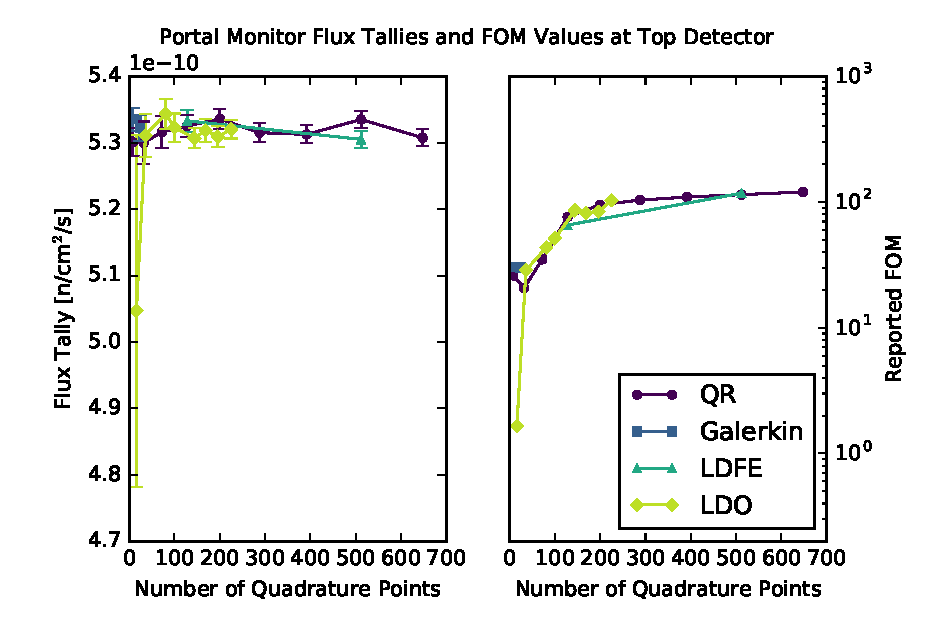
\includegraphics[max height=0.445\textheight]
{portal-fwcadis-1.eps}
\subcaption{MCNP-reported forward flux tally and FOM values at the top detector.}
\end{subfigure}
\\
\begin{subfigure}{\textwidth}
\centering
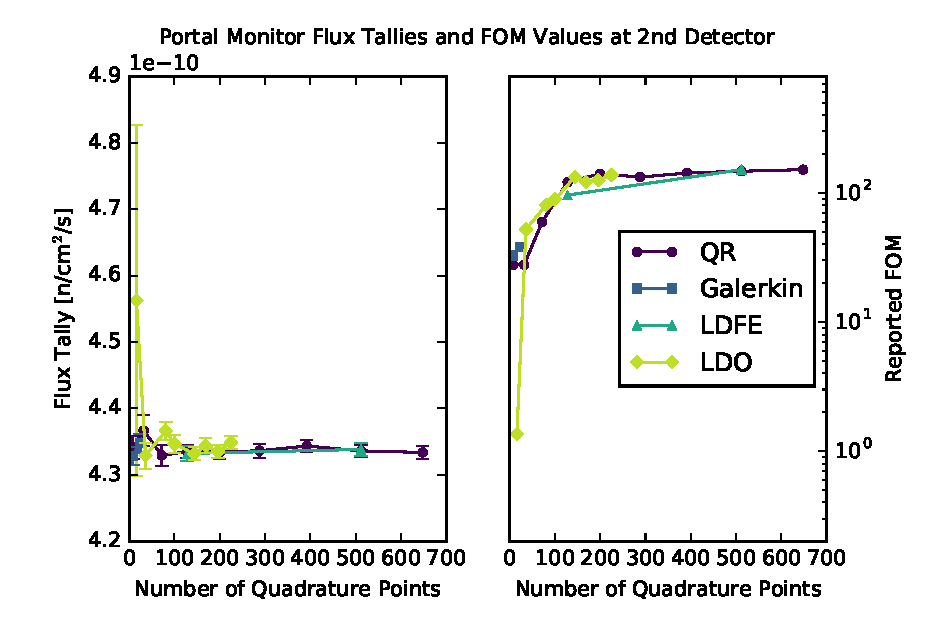
\includegraphics[max height=0.445\textheight]
{portal-fwcadis-2.eps}
\subcaption{MCNP-reported forward flux tally and FOM values at the second detector.}
\end{subfigure}
\end{figure}
\clearpage
\begin{figure}[!htb]
\ContinuedFloat
\begin{subfigure}{\textwidth}
\centering
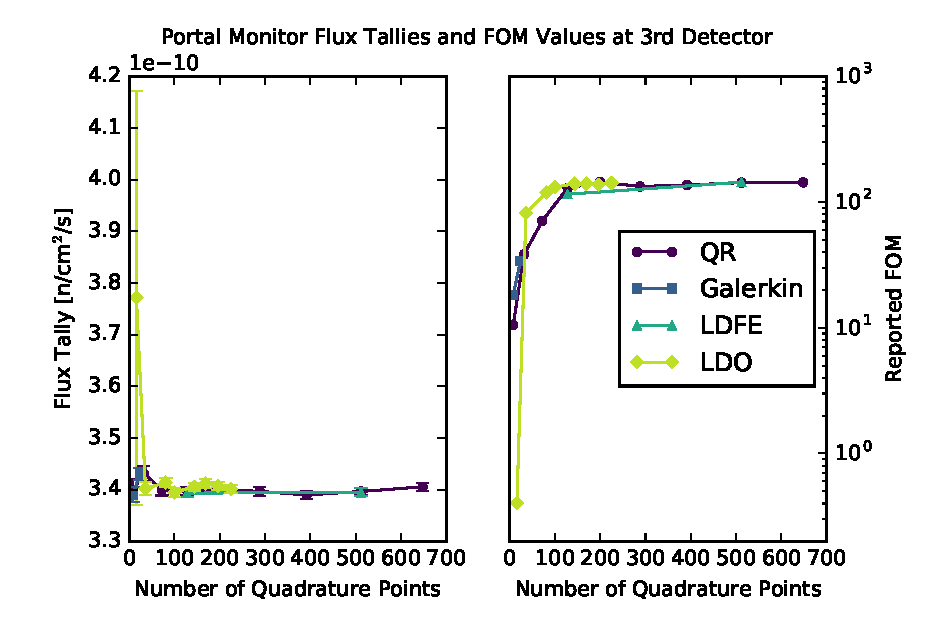
\includegraphics[max height=0.445\textheight]
{portal-fwcadis-3.eps}
\subcaption{MCNP-reported forward flux tally and FOM values at the third detector.}
\end{subfigure}
\\
\begin{subfigure}{\textwidth}
\centering
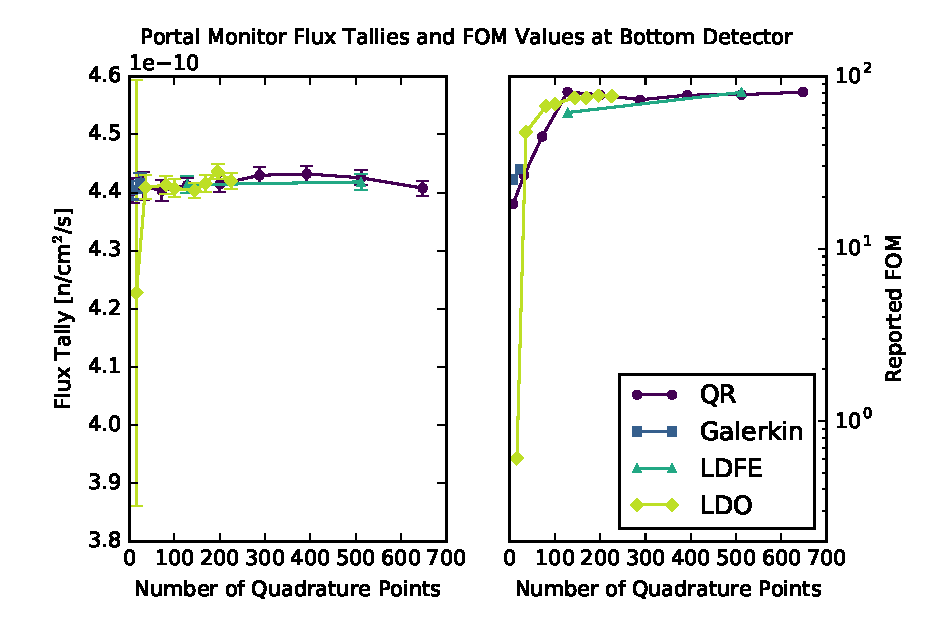
\includegraphics[max height=0.445\textheight]
{portal-fwcadis-4.eps}
\subcaption{MCNP-reported forward flux tally and FOM values at the bottom detector.}
\end{subfigure}
\caption{\fwc\ flux tallies and FOM values for the portal monitor scenario.}
\label{cargo-fwc}
\end{figure}

\FloatBarrier
%%---------------------------------------------------------------------------%%
\subsection{Summary}

In this work, we tested the use of LDO quadrature sets in CADIS and \fwc\ for
problems with challenging angular streaming behavior. These real engineering
problems are difficult for any Monte Carlo solver, and we set out to identify
if the angular properties of the LDO equations could provide an advantage over
traditional \sn\ quadratures. The LDO equations saw their best-performing
Monte Carlo VR parameters in the \fwc\ context, where the LDO formulation's
angular information is better incorporated into the variance reduction
parameter generation.

In the context of the \fwc\ method, we found that low-order (5 or 8) angular
meshes (36 to 81 discrete ordinates) are sufficient to produce forward flux
tally and Figure of Merit values comparable to those of more refined angular
meshes when using LDO quadrature sets. The superior FOM values resulting from
the representative LDO quadrature set for three of four detectors in the
simplified portal monitor scenario begets interest in further exploration of
LDO equations' solutions as input for Monte Carlo VR parameters for photon
transport in the \fwc\ context.

On the whole, little correlation was seen between angular mesh refinement and
the MCNP-reported forward flux tally values in the CADIS context. If using an
LDO quadrature set to generate variance reduction parameters in this context
for any of the neutron transport problems, a low-order (3 to 8) quadrature
set (16 to 81 discrete ordinates) may be used to sufficient effect for flux
tally value and FOM achievement. For generating VR parameters in the CADIS
context for a photon problem with an LDO quadrature set, the finest available
angular mesh should be used. This is consistent with what is expected based on
the difference between neutron and photon scattering in the materials in these
test cases.

%---------------------------------------------------------------------------%%
\section{Conclusions and Future Work}
\label{sec:conclusions}

Hybrid methods can be highly effective in allowing the use of Monte Carlo
methods to solve tough shielding problems. However, for engineering problems
with streaming paths and strong anisotropies, such as steel embedded in water or
concrete, and small air gaps between shielding materials, CADIS and \fwc\ are
ineffective at getting low enough relative error in the regions of streaming.
The LDO formulation offers lesser ray effects, superior mathematical properties,
and more flexible angular treatment than the classical \sn\ equations for an
equivalent number of angles. We investigated whether using LDO for VR parameter
creation was more effective than standard quadratures.

The LDO equations saw their best-performing Monte Carlo VR parameters in the
\fwc\ context. This makes sense as the LDO formulation is capturing better
overall performance than equivalent \sn\ constructions, which will be reflected
in global VR. The LDO formulation does not improve localized performance as
much, so we therefore do not expect CADIS to see as much improvement.

For the DLVN experimental benchmark, LDO variance reduction
parameters generated the highest Figures of Merit for two of the six detector
locations in the assembly. Of those studied here, the only other quadrature
type to achieve this was the QR quadrature set. In the case of the simplified
portal monitor scenario studied in the \fwc\ context, the LDO VR
parameters attained the highest FOM values for three out of four detector
locations. Considering results from the test cases in which neutrons
were transported using the CADIS and \fwc\ methods, we suggest a coarse
angular mesh for Monte Carlo variance reduction parameter generation based on
flux solutions resulting from solving the LDO equations. For photon transport
problems, a more refined LDO angular mesh is recommended for generating Monte
Carlo VR parameters and achieving detector responses with high Figures of
Merit.

In general, the LDO formulation is most useful in the specific context of Monte
Carlo variance parameter generation using the \fwc\ method for photon transport
problems. It is also effective in the \fwc\ method for neutron transport
problems, though somewhat less so. Overall, LDO was more effective than
equivalent \sn-created VR parameters for a variety of standard quadratures for
these tough engineering problems containing streaming behaviors that are
difficult for hybrid methods to capture.

The LDO representation
is currently limited in applicability by its current implementation in the
Exnihilo framework and the ADVANTG software. The problem space available to
explore is limited to those with vacuum boundary conditions and isotropic
fixed particle sources with non-zero volume. It would be useful to test a
wider variety of sources, and using other boundary condition types could speed
up calculation times.

An additional area of research that could prove interesting comes from the
flexibility of the LDO equations. In this work we did not specifically adapt
the angles of evaluation to the problems of interest. For example, one could
use the interpolatory nature of the LDO formulation to cluster angles along
the direction of streaming paths. It could be that increased angular resolution
in key directions could improve performance of the VR parameters generated.
The purpose of this work, however, was a first evaluation of using LDO
solutions for Monte Carlo variance reduction and in doing so we identified several areas of valuable application. 

\pagebreak
\section*{Acknowledgments}

This material is based upon work supported under an Integrated
University Program Graduate Fellowship as well as supported by the Department 
of Energy under Award Number(s) DE-NE0008661. This report was prepared as an
account of work sponsored by an agency of the United States Government.
Neither the United States Government nor any agency thereof, nor any of their
employees, makes any warranty, express or limited, or assumes any legal
liability or responsibility for the accuracy, completeness, or usefulness of
any information, apparatus, product, or process disclosed, or represents that
its use would not infringe privately owned rights. Reference herein to any 
specific commercial product, process, or service by trade name, trademark, 
manufacturer, or otherwise does not necessarily constitute or imply its 
endorsement, recommendation, or favoring by the United States Government or
any agency thereof. The views and opinions of authors expressed herein do not 
necessarily state or reflect those of the United States Government or any 
agency thereof. This research used the Savio computational cluster resource 
provided by the Berkeley Research Computing program at the University of 
California, Berkeley (supported by the UC Berkeley Chancellor, Vice Chancellor
for Research, and Chief Information Officer).

\pagebreak

\bibliographystyle{nse}
\bibliography{ldo-mc-vr}

\end{document}

